%%%%%%%%%%%%%%%%%%%%%%%%%%%%%%%%%%%%%%%%%%%
%THIS FILE CONTAINS ALL COMMON COMMANDS NEEDED FOR COMPILATION INTO BOTH PDF AND HTML.
%THE EXTENSION file src/macros.sty CONTAINS ONLY COMMANDS NEEDED EXCLUSIVELY FOR COMPILATION INTO PDF
%THE DIRECTORY src/hva/ CONTAINS ONLY COMMANDS NEEDED EXCLUSIVELY FOR COMPILATION INTO HTML WITH HEVEA, WITH THREE EXTENSION FILES, imakeidx.hva, macros.hva AND picins.hva.
%%%%%%%%%%%%%%%%%%%%%%%%%%%%%%%%%%%%%%%%%%%
% 2024/04:
% - \documentclass[] : change {book} to {scrbook} from KOMA-script -> rewritting the manual.
% - change fancyhdr to scrlayer-fancyhdr (compatibility with scrbook) to scrlayer-scrpage (contained in koma-script) -> modify macros.sty too.
% - rewriting title page for \maketitle (use with pandoc [produce html file], \begin(title)...\end(title) doesn't work with pandoc, "microtype" package too)
% 2024/10
% - renaming chapter files with an order number
% - clean documentclass / packages / add comments
% 2024/10
% - comment \ifIllustration to always have pictures in manuel
% - texlive-extra-utils -> make4ht
% 2024/11
% - simplification of \usepackage{graphicx} when pdf

\documentclass[%
	pdflatex,
	a4paper,			% default=a4 and therefore not needed
	12pt,				% default=11pt
	french,				% use in babel, translator and varioref packages options %TODO: change with ngerman/english option in de/en manuals
	toc=listof,			% add a "lof" (list of figures) line at the begining of the toc (table of contents)
	twoside=semi,		% same recto/verso margins similar to simple verso margins, default=twoside
	headsepline,		% draw rule below header
	footsepline,		% draw rule above footer
	plainfootsepline 	% draw footsepline on plain pages (here for heading pages, may be due to twoside=semi in scrbook options
]{scrbook} 				% KOMA-Script class "book"		


\usepackage[T1]{fontenc}			% the font encoding
%\usepackage[utf8]{inputenc}			% no longer need to specify, included in LaTex since April 2018
\usepackage{lmodern}				% Latin Modern police
\usepackage{babel}					% use the language define in \documentclass
\def\frenchcontentsname{Sommaire}	% rename "Table des matières" (at end of document) from [french]{babel} to "Sommaire" (at start of document)
\frenchsetup{ItemLabeli=\textbullet}		% change 1st level list marker of french babel
\frenchsetup{ItemLabelii=\textopenbullet}	% change 2nd level list marker of french babel
\usepackage{translator}				% for translating the Fixed Names
\usepackage{textcomp}				% for special characters like \textcurrency
\usepackage{newtxtext}				% install texlive-fonts-extra, replacing times which replaces txfonts
%\usepackage{lwarp}					% produce html file with lwarp (install texlive-extra-utils)
\usepackage[letterspace=200]{microtype}				% Font expansion (use for title) with "\textls[x]" - doesn't work with pandoc / espace entre caractères (utilisé pour le titre)
\usepackage{graphicx}				% enhanced support for importing graphics (x=enhanced) and then using the \includegraphics command to insert the file
\newcommand{\refimage}[1]{ (fig. \vref{#1})}	% for the hypertext link display on images
\newcommand{\vspacepdf}[1]{\vspace{#1}}			% for spaces after images bordered with text

% For illustrations
%\usepackage{picins}				% for text around image TODO change to wrapfig2 in the manuel
\usepackage{wrapfig2}				% TODO change in chapters, for text around image (replace picins)
\usepackage{caption}				% for good references in table of figures

\usepackage{varioref}				% defines the commands \vref, \vpageref, \vrefrange, and \vpagerefrange in french
\usepackage{color}					% for a colored title page
\usepackage{thumbpdf}				% create thumbnails (vignettes) in pdf

%% Page layout %%
\usepackage[%
%	showframe,					% to see frame of geometry package
	top=1in,					% marge haute
	headheight=7mm,				% hauteur en-tête
	headsep=6mm,				% distance entre entête et corps de texte
	textheight=252mm,			% textheight=paperheight-topmargin-headheight-headsep-footskip
	footskip=11mm,				% distance entre bas de pied de page et bas du corps de texte
	hmargin=25mm				% horizontal margins (left and right), textwidth = paperwidt - margins
]{geometry}
\usepackage{scrlayer-scrpage}	% define and manage page styles by controlling page headers and footers			
\clearpairofpagestyles			% remove the default marks of the headings and the plain pages
\lehead{\leftmark}				% leftmark at left of even page
\lohead{\leftmark}				% leftmark at left of odd page
\rehead{\rightmark}				% rightmark at right of even page
\rohead{\rightmark}				% rightmark at right of odd page
\cfoot*{\pagemark}				% pagemark in the center of the footer
\ModifyLayer[addvoffset=-1ex]{scrheadings.foot.above.line}		% shift line up to increase distance between footer text and footerline in normal stylepages
\ModifyLayer[addvoffset=-1ex]{plain.scrheadings.foot.above.line}	% shift line up to increase distance between footer text and footerline in plain style page (chapter page)

%% Footnotes %%
\usepackage[%
	perpage						% resets footnote numbering for each page of the document.
]{footmisc}						% provides several different customizations of footnotes

\renewcommand\footnoterule{%	% redefine rule above footnote
	\kern 5pt 					% above footnoterule, space between text and footnoterule  
	\hrule width 2.5in			% define rule's width to 2.5 in
	\kern 6pt					% space between footrule and footnotes below
}

%% Table of Contents (toc) %%
\setcounter{tocdepth}{1}		% modifies the depth of the toc (default=2)

%% Index %%
\usepackage[%
	xindy						% sort index
]{imakeidx}						% for creating an index
\usepackage[%
	columns=2,					% default value is 2
	rule=1pt,					% thickness of a vertical rule between index columns. Default value is 0 pt, i. e. no rule.
	totoc						% add index in toc
]{idxlayout}					% key-value interface to configure index layout parameters


\usepackage[unicode]{hyperref}			% replace \usepackage{url}, used to add an URL and rewrite the "grisbi-manuel-urldef.tex" file (must be the last package)
\hypersetup{%							% to create metadata to insert in pdf
	pdftitle={Manuel de Grisbi},		% sets the document information Title field
	pdfauthor={The Grisbi Team},		% sets the document information Author field
	pdfcreator={Alain PORTAL}			% sets the document information Creator field
	pdfpagemode=UseOutlines,			% set default mode of PDF display, UseOutlines=show bookmarks
	pdfstartview=XYZ null null 1.0,		% set the startup page view, XYZ=left top zoom
	pdffitwindow=true,					% resize document window to fit document size, default=false
	pdfcenterwindow=true,				% position the document window in the center of the screen, default=false
	bookmarksnumbered=true,				% put section numbers in bookmarks, default=false
	bookmarksopen=true,					% open up bookmark tree, default=false
	colorlinks=true,					% color links, default=false
	citebordercolor=1 1 1,				% the color of the box around citations, rgb color
	linkbordercolor=1 1 1,				% the color of the box around normal links, rgb color
	linkcolor=blue,						% color for normal internal links, color=blue
	menubordercolor=1 1 1,				% color of border around menu links, rgb color
	urlbordercolor=1 1 1,				% color of border around URL links, rgb color
	urlcolor=blue,						% color of URL links, color=blue
	plainpages=true						% do page number anchors as plain Arabic, default=false
%	pdfpagelabels=true					% set PDF page labels - Commenté car élimine  "Package hyperref Warning: Option `pdfpagelabels' has already been used,"
}
\include{31-grisbi-manuel-urldef}		% include the "grisbi-manuel-urldef" file during the compilation

%% Glossary %%
\usepackage[%
	xindy,				% sort glossaries
	toc                 % add the glossary reference to the toc (table of contents)
]{glossaries}			% create a glossary, must be loaded AFTER hyperref
\usepackage[%
	automake
]{glossaries-extra} 	% check why no glossaries and give solutions

%% Index %%
\makeindex  %[intoc]	% creates the index with its reference in the toc

\definecolor{jaunegrisbi}{rgb}{1,1,.6}			% creating your own colors {yourcolorname}{model=rgb[0to1],RGB[0to255],cmyk or grey} rgb= 3 comma-separated values between 0 and 1 define the components of the color.
\definecolor{bleugrisbi}{rgb}{.1,.1,.4}
\definecolor{vertgrisbi}{rgb}{0,.6,.4}
\definecolor{ocregrisbi}{rgb}{1,.7,0}

% Virtualization of fonts
\newcommand{\lang}[1]{\emph{#1}}				% new command -> \lang = emph (e.g. italic)
\newcommand{\familyname}[1]{\textsc{#1}}		% new command -> \familynamelang = small caps
\newcommand{\menu}[1]{\textsl{#1}}				% new command -> \menu = slanted is oblique version of the roman font (e.g. italic)
\newcommand{\strong}[1]{\textsc{\textbf{#1}}}	% new command -> \strong = small caps + bold
\newcommand{\key}[1]{\texttt{<#1>}}				% new command -> \key = teletype font
\newcommand{\cmd}[1]{\texttt{#1}}				% new command -> \cmd = teletype font
\newcommand{\file}[1]{\textbf{#1}}				% new command -> \file = bold
\newcommand{\xml}[1]{\texttt{#1}}				% new command -> \xml = teletype font
\newcommand{\indexword}[1]{\textsf{#1}}			% new command -> \indexword = sans serif, for easy search of each indexed word in the page

\newcommand{\actuality}{}						% to see places to watch when updating the doc, using  the command grep actuality *.tex

% Glossary
\makeglossaries									% creates the glossary, entries of the glossary are in "src/{version}/{lang}/30-grisbi-manuel-glossary.tex"

%\input{grisbi-manuel-glossary}					% include "grisbi-manuel-glossary.tex" file in the document
\loadglsentries{30-grisbi-manuel-glossary}		% load and include glossary's entries in and from "30-grisbi-manuel-glossary"

\begin{document}

%% -------------------
%% Begin of title page
%% -------------------
\begin{titlepage}
	\title{Manuel de Grisbi}						% to avoid "[WARNING] This document format requires a nonempty <title> element" with pandoc
	\subtitle{Logiciel de comptabilité personnelle et associative}%
	\begin{center}
	\sffamily										% sans serif (or rmfamily(roman) or ttfamily(“typewriter”))
	\bfseries										% bold (or mdseries(regular))
	\fontsize{40}{48}\selectfont					% increase size to 40pt / line spacing=48pt
	\scshape										% small caps
%	M\:a\:n\:u\:e\:l\; d\:e\; G\:r\:i\:s\:b\:i\par	% \: = medium space, \; = large space, \\ = line break
%	\textls[200]{%									% increase space between characters, default=100 (active "microtype" package) [[ !!! doesn't work with pandoc !!! ]]
	\lsstyle										% defined with the ‘letterspace’ option in the microtype package
	Manuel de Grisbi
	\end{center}
	\begin{center}
	\vspace{1.8cm}
	\includegraphics[width=6cm]{image/grisbi-logo.png}\par		% insert {file_name} graphic with width=6cm
	\vspace{1.8cm}									% vertical space between logo and subtitle
	\end{center}
	\begin{center}
	\sffamily										% without serif
	\bfseries										% bold
	\scshape										% small caps
	\fontsize{19}{22}\selectfont					% increase size to 19pt / line spacing=22pt
	Logiciel de comptabilité personnelle et associative
	\vspace{.8cm}									% vertical space
	\end{center}
	\begin{center}
	\rule{4.5cm}{0.4pt}\par							% horizontal line, first argument width, second thickness
	\vspace{1.6cm}									% vertical space
	\end{center}								
	\begin{center}
	\rmfamily										% roman
	\mdseries										% regular
	\large											% font size
	Copyright © 2001-2003 Daniel \familyname{Cartron}\\
	Copyright © 2004 Loïc \familyname{Breilloux}\\
	Copyright © 2004 Benjamin \familyname{Drieu}\\
	Copyright © 2011-2014 Jean-Luc \familyname{Duflot}\\
	Copyright © 2018 Bob \familyname{Anderson} (en)\\
	Copyright © 2018-2020 Martin \familyname{Stromberger} (de)\\
	Copyright © 2024-2025 Dominique \familyname{Brochard}\par
	\vspace{.3cm}
	\rule{2.5cm}{0.4pt}\par							% insert horizontal line, first argument width, second thickness
	\vspace{.5cm}
	Version 3.0 de 2025 (provisoire)
	\end{center}
\end{titlepage}

\frontmatter						% rend les pages numérotées du sommaire/table des figures en minuscules romaines / renders numbered pages in toc/tof in lower-case Roman letters

%\sommaire
\tableofcontents					% table of contents (toc)	

\listoffigures						% list of figures (lof)

\mainmatter								% la numérotation des pages se fait en chiffres arabes et le compteur de pages est remis à 1 / pages are numbered in Arabic numerals and the page counter is reset to 1.
%\KOMAScriptVersion						% print the used version number of Koma-Script

%%%%%%%%%%%%%%%%%%%%%%%%%%%%%%%%%%%%%%%%%%%%%%%%%%%%%%%%%%%%%%%%%
% Contents: The preamble chapter
% $Id: grisbi-manuel-preamble.tex, v 0.4 2002/10/27 Daniel Cartron
% $Id: grisbi-manuel-preamble.tex, v 0.6.0 2011/11/17 Jean-Luc Duflot (no change)
% $Id: grisbi-manuel-preamble.tex, v 0.8.9 2012/04/27 Jean-Luc Duflot (typo changes)
% $Id: grisbi-manuel-preamble.tex, v 1.0 2014/02/12 Jean-Luc Duflot
% $Id: grisbi-manuel-preamble.tex, v 3.0 2024/04/10 Dominique Brochard: writing the Préambule in the 3rd person (Daniel Cartron). Add Blu-ray zone 2 and DVD/Blu-ray zone 1.
%%%%%%%%%%%%%%%%%%%%%%%%%%%%%%%%%%%%%%%%%%%%%%%%%%%%%%%%%%%%%%%%%

% supprimé car inopérant en pdf et crée un problème en html
%\begin{small}

%commande étoilée : étoile supprimée pour entrées d'index avec affichage du lien correct en html
\chapter{Préambule\label{preamble}}

%% commenté pour entrées d'index avec affichage du lien correct en html
%% voir aussi le chapitre préambule déplacé dans le \mainmatter dans manuel.tex
%\markboth{}{Préambule}
%\ifpdf
%\addcontentsline{toc}{chapter}{Préambule}
%\else
%\fi

Plusieurs utilisateurs de \gls{Grisbi} ont demandé à Daniel \familyname{Cartron} d'insérer dans le manuel un bref rappel de la signification de ce mot, qui, à son grand dam, est retombé en
désuétude.

Ses premières (brèves) recherches n'ayant pas ramené de résultats valant la peine d'être publiés, il avait laissé tomber jusqu'à ce qu'un jour il prenne le temps de passer quelques moments dans une bibliothèque bien fournie en dictionnaires de toutes sortes. Et là, la moisson fut abondante. Tellement abondante que Daniel \familyname{Cartron} hésité longuement pour savoir ce qu'il allait garder et ce qu'il allait éliminer\ldots

Finalement il décida de tout garder, même si on passe ainsi à un paragraphe de quatre pages. Il a juste opéré un classement des articles les plus courts vers les plus longs.

En effet il trouve intéressant d'étudier les divergences entre les différents
dictionnaires, mais plus encore de constater les ressemblances, à ce point
frappantes que l'on pourrait intituler ce chapitre non pas \emph{Le jeu des sept
erreurs} mais \emph{Qui a copié qui?} À vous de trouver\dots

Et il a aussi rajouté un passage sur le film puisque pour ceux qui savent encore
ce que \indexword{grisbi}\index{Grisbi} veut dire cela tient essentiellement à la renommée méritée de cette \oe uvre.


\section{Étymologie\label{preamble-etymology}}


Voici donc quelques sources sur l'étymologie\index{etymologie@étymologie} du mot grisbi :


\subsection*{Dictionnaire de la langue française --- Hachette}

[grizbi] n. m. Arg. Argent --- De gris (monnaie grise ; cd. rouchi griset [1834], \frquote{liard}), et suff. pop. -bi ; 1895, répandu en 1953.


\subsection*{Grand Larousse de la langue française}

[grizbi] n. m. (de \emph{gris[et]}, pièce de six liards [1834, Esnault] --- dér.
de \emph{gris}, à cause de la couleur [cf. aussi \emph{grisette}, \frquote{monnaie} --- XVIIe s. ---, et \emph{monnaie blanche et grise}, 1784, Esnault] --- avec le suff.arg. \emph{-bi} ; 1896, Delesalle).

\emph{Arg.} Argent : \emph{Touchez pas au grisbi} (titre d'un roman d'Albert
Simonin [1953]).


\subsection*{Dictionnaire historique de la langue française --- Robert}

n.m. apparu en 1895 (\emph{grisbis}) et répandu à partir de 1953 par le roman
\emph{Touchez pas au grisbi} de A. Simonin, serait composé de \emph{gris}
\frquote{ monnaie grise} (1784 : cf. le rouchi \emph{griset} \frquote{pièce de six liards}, 1834 ; et \emph{grisette} \frquote{monnaie}, v. 1634) et de l'élément \emph{bi} d'origine obscure : \emph{grisbi}, \frquote{argent} en argot, pourrait être un composé tautologique de \emph{gris} et \emph{bis}.


\subsection*{Dictionnaire de l'argot français et de ses origines --- Larousse}

Origine très controversée : soit de griset, \frquote{pièce de monnaie}, et d'un
mystérieux suffixe -bi, ou du pain à la fois gris et bis, ou du slang anglais
crispy, argent ; nous proposons d'y voir un emploi métonymique de gripis 1628
[Cheneau], grispin, grisbis 1849 [Halbert], \frquote{meunier}, c'est-à-dire \frquote{celui qui a chez lui du blé} 1895 [Delsalle] mais remis en circulation par \frquote{Touchez pas au grisbi}, célèbre roman de A. Simonin, paru en 1953.

VARIANTES ---  grijbi : 1902 [Esnault] --- grèzbi : vers 1926 [id.]

DÉRIVÉS --- grisbinette n.f. Pièce de cent anciens francs : 1957
[Sandry-Carrère].


\subsection*{Trésors de la langue française}

\emph{Arg.} Argent. Synon. pop. \emph{fric, galette, pèze, pognon. Le grisbi je suis assez grand pour aller le chercher moi-même ! (\ldots) Riton qu'avait même pas su se tenir en homme (\ldots) dès qu'il s'était senti assez de grisbi} (\familyname{Simonin}, \emph{Touchez pas au grisbi}, 1953, p. 231).

\strong{Prononc.} : [grizbi].  \strong{Étymol. et Hist.} 1896 \emph{grisbis}
arg. \frquote{argent} (\familyname{Delesalle}, \emph{Dict. arg.-fr. et fr.-arg.}). Mot composé du rad. de \emph{griset}, au sens de \frquote{pièce de six liards} (1834 ds \familyname{Esn.}), dér. de \emph{gris}, à cause de la couleur (\emph{cf.} aussi \emph{ca} 1634 \emph{grisette} \frquote{monnaie}, \emph{La Muse Normande} de D. Ferrand, éd. A. Héron, II, 91 ; 1784, Brest, \emph{monnaie blanche et grise} ds \familyname{Esn.}), et d'une seconde partie d'orig. obsc. qui représente peut-être le suff. pop. -bi, à rapprocher de \emph{nerbi} \frquote{très noir} (d'apr. \familyname{Esn.}). Il n'est pas impossible que \emph{grisbi} (anciennement \emph{grisbis}) soit un composé tautologique de \emph{gris} et de \emph{bis}.
\strong{Bbg.} \familyname{Rigaud} (A.). L'arg. litt. \emph{Vie lang.} 1972, pp. 114-117.


\subsection*{Grand Robert de la langue française}

[grizbi] n. m. --- 1895 : répandu 1953 par le roman de Simonin \emph{Touchez pas au grisbi} ; le mot était rare ou archaïque v. 1950 : de \emph{gris} \frquote{monnaie grise} (cf. rouchi \emph{griset} \frquote{liard}, 1834), et suff. pop. \strong{Argot.} Argent. \emph{T'as du grisbi ?}

1 --- Cette expression : \frquote{Ne touchez pas au grisbi} devient une variante de \frquote{Ne chahutez pas avec les nippes}. C'est le maître mot qui dirige la chronique de ces chevaliers de fortune mal acquise qui donnèrent de la mobilité aux romans de cape et de mitraillette de Peter Cheyney.

			\familyname{P. Mac Orlan}, \emph{in} Albert \familyname{Simonin}, Touchez pas au grisbi, Préface, p. 6.

2 --- \frquote{Te casse pas la tête pour les politesses\ldots{ } D'abord on a pas le temps si tu veux que je te trouve Ali. Tout dépend de ce qu'il a de grisbi en fouille ; s'il est armé, on a une chance de le trouver au flambe, à la partie du Carillon}

			Albert \familyname{Simonin}, Touchez pas au grisbi, p. 147.


\subsection*{Dictionnaire du français non conventionnel --- Hachette}

n.m. (grisby)

Argent (intrinsèquement).

\emph{Au petit caïd de l'équipe, un mouflet à casquette torpédo, bleu de
chauffe et pompes vernies, la môme venait d'affirmer qu'elle me frimait
seulement pour le bon motif, pour me soulager de mes cent sacs. Il avait
répliqué, le vilain jalmince :
--- Le \emph{grisbi}, je suis assez grand pour aller le chercher moi-même !
Ils disaient vrai tous les deux, l'un et l'autre également prêts à tout pour le
\emph{grisbi}. Eux et leurs petits potes. Pareil Angelo-la-Tante et
Josy-la-Peau-de-Vache ; pareil Ali-le-Fumier et ses ordures d'espingos ;
pareil Riton qu'avait même pas su se tenir en homme avec sa môme, dès qu'il
s'était senti assez de \emph{grisbi} ; pareil Marco et sa petite Wanda, si
honnête, mais qu'hésitait pas à se faire enjamber par le bonhomme \emph{grisbi} ! pareil aussi la môme Lulu sans doute, qu'attendait patiemment chez moi que je rabatte, avec mon \emph{grisbi} !}

			A. \familyname{Simonin}, Touchez pas au grisbi, p. 233

HIST. ---1895, mais sans doute peu usité : A. Bruant et L. Blédort, qui
accumulent à l'occasion les synonymes (\emph{pèse, os,} etc.), n'emploient pas \emph{grisbi}, bien que Bruant l'enregistre en 1901 (\emph{grisbis}). Le succès mérité du roman d'A. Simonin en 1953 a rendu une jeunesse au mot, qui ne paraît pas pour autant véritablement intégré à la série des désignants de l'argent, comme \emph{blé, oseille, flouze} ou \emph{fric}.

Du rouchi \emph{griset}, \frquote{pièce de six liards} (1834), ainsi dénommée à cause de sa couleur. Mais l'explication donnée par Esnault, actuellement seule 
disponible, n'est pas satisfaisante ; d'une part, l'élément \emph{bi} reste
inexpliqué, sinon par un \frquote{suffixe} inconnu ; d'autre part, Bruant écrit
\emph{grisbis}, et il est possible (sinon probable) que le \emph{s} central ne
soit prononcé que depuis 1953 ; ce qui amènerait à une explication :
\emph{gris-bis}, dans la série des désignants issus d'un nom du pain,
\emph{blé, carme, biscuit, galette}, etc.

Enfin, si la métonymie de la couleur est effectivement utilisée pour dénommer
l'argent, il s'agit toujours d'une catégorie d'argent précise : des \frquote{espèces}.
Ainsi \emph{jaunet, blanc, blanche, cuivre}, ne sont pas interchangeables, ni 
utilisables pour \frquote{de l'argent} abstrait.

On rappellera par ailleurs le sens de \emph{gris} : \frquote{cher} (V. \emph{grisol}) et la possibilité du pseudo-suffixe augmentatif \emph{bi}, \frquote{très}, même rare. On aurait alors : \emph{gris-bi}, \frquote{très cher} ? Mais l'hypothèse est aventurée.


\section{Bibliographie\label{preamble-biblio}}


\emph{Touchez pas au Grisbi !} par Albert \familyname{Simonin}

\begin{itemize}
	\item Gallimard, Folio Policier \no 183, 1ère édition en 1953, réédition en 2014 (toujours édité)
	\item Gallimard, Folio \no 2068, première édition en 1989
	\item Gallimard, Carré Noir \no 94, première édition en 1972
	\item Le Livre de Poche \no 1152, première édition en 1953
	\item Gallimard, Série Noire \no 148, première édition en 1953
\end{itemize}


\section{Filmographie\label{preamble-filmography}}


\strong{Touchez pas au grisbi !}

Film italien, français (1953). Policier. Durée : 1h 34 min

Titre Original : Grisbi

Distribution :

\begin{itemize}
	\item Jean \familyname{Gabin} : Max le menteur	
	\item René \familyname{Dary} : Riton ;
	\item Dora \familyname{Doll} : Lola	
	\item Vittorio \familyname{Sanipoli} : Ramon	
	\item Marilyn \familyname{Buferd} : Betty	
	\item Gaby \familyname{Basset} : Marinette	
	\item Paul \familyname{Barge} : Eugène
\end{itemize}

Réalisateur : Jacques \familyname{Becker}


\subsection*{Synopsis}

Max-le-menteur et Riton viennent de réussir le coup de leur vie : voler 50
millions de francs en lingots d'or à Orly. Avec ce \frquote{grisbi}, les deux
gangsters comptent bien profiter d'une retraite paisible. Mais Riton ne peut
s'empêcher de parler du magot à sa maîtresse Josy. L'entraîneuse transmet la
précieuse information à Angelo, un trafiquant de drogue avec lequel elle trompe Riton. Angelo kidnappe le vieux truand et demande le \frquote{grisbi} à Max comme rançon\dots


\subsection*{Anecdotes}

\paragraph{Un tandem bien huilé :} Jean \familyname{Gabin} et René 
\familyname{Dary} sont considérés comme deux monstres sacrés du cinéma de
l'avant-guerre.

\paragraph{\familyname{Becker} père et fils :} Le fils de Jacques 
\familyname{Becker}, Jean, fait ici ses débuts au cinéma en tant qu'assistant
réalisateur. Il n'a pourtant que quinze ans !

\paragraph{Albert \familyname{Simonin} :} L'écrivain et scénariste Albert
\familyname{Simonin}, qui adapte ici son propre roman, fera quatre autres films avec \familyname{Gabin}, tous dialogués par \familyname{Audiard} : \emph{Le cave se rebiffe} (1961) et \emph{Le gentleman d'Epsom} (1962) de Gilles \familyname{Grangier}, \emph{Mélodie en sous-sol} (1963) d'Henri 
\familyname{Verneuil} et \emph{Le pacha} (1967) de Georges \familyname{Lautner}. Après avoir adapté son \oe uvre \emph{Les Tontons flingueurs} pour Georges \familyname{Lautner} (1963), il devient son scénariste pour \emph{Les Barbouzes}
(1964).


\subsection*{Version DVD zone 2}

\begin{itemize}
	\item Interactivité : Menu d'accueil, accès aux scènes, filmographies déroulantes du réalisateur, de Lino \familyname{Ventura} et Jean \familyname{Gabin}
	\item Format cinéma : plein écran
	\item Version sonore : VF en mono
	\item Sous-titres : aucun
	\item France --- 1953 --- Noir \& blanc --- 92 min --- Film Office --- 1~disque --- 1~face --- 1~couche
	\item Date de parution : 19 septembre 2001
	\item Éditeur : Studio Canal
\end{itemize}

\subsection*{Version Blu-ray zone 2}

\begin{itemize}
	\item Format cinéma : 4/3 format respecté 1.33
	\item Version sonore : VF en stéréo
	\item France --- 1953 --- Noir \& blanc --- 94 min
	\item Sous-titres : aucun
	\item Date de parution : 10 mars 2017
	\item Éditeur : Studio Canal
\end{itemize}

\subsection*{Versions DVD / Blu-ray zone 1}

Les versions zone 1 contiennent des sous-titres en anglais, avec en plus, des interviews des acteurs.
% supprimé car inopérant en pdf et crée un problème en html
%\end{small}
				% TODO: update screenshots and text "preamble", remove % when finished
%\cleardoubleemptypage

%%%%%%%%%%%%%%%%%%%%%%%%%%%%%%%%%%%%%%%%%%%%%%%%%%%%%%%%%%%%%%%%%
% Contents : The introduction chapter
% $Id : grisbi-manuel-intro.tex,v 0.4 2002/10/27 Daniel Cartron
% $Id : grisbi-manuel-intro.tex, v 0.5.0 2004/06/01 Loic Breilloux
% $Id : grisbi-manuel-intro.tex, v 0.6.0 2011/11/17 Jean-Luc Duflot
% $Id : grisbi-manuel-intro.tex, v 0.8.9 2012/04/27 Jean-Luc Duflot
% $Id : grisbi-manuel-intro.tex, v 1.0 2014/02/12 Jean-Luc Duflot
% $Id : grisbi-manuel-intro.tex, v 3.0 2024/11 Dominique Brochard :
% - update links and text
% - update pdf/html readers
% - add versions 0.1 to 0.4.4
% - use \label within \footnote command, and after use \footref to avoid duplicates in footnotes
% - add newsgroups in 2.4 Contacts
%%%%%%%%%%%%%%%%%%%%%%%%%%%%%%%%%%%%%%%%%%%%%%%%%%%%%%%%%%%%%%%%%

\chapter{Introduction\label{introduction}}


\section{Généralités\label{introduction-general}}


Grisbi est un \gls{logiciel libre} de comptabilité personnelle, développé en \gls{Langage C} avec le support \gls{GTK}+ 3, originellement pour la plate-forme \gls{GNU/Linux}. Il y a maintenant un \indexword{\gls{portage}}\index{portage} sous \gls{Windows}, \gls{macOS}, FreeBSD, des paquetages pour différentes \gls{distributions Linux}, et d'autres possibilités à découvrir sur le site de \lang{Grisbi}\footnote{\urlGrisbi{}} ou celui de \lang{Sourceforge}\footnote{\urlSourceForge{}}.

Le principe de base est de vous permettre de classer de façon simple et intuitive vos opérations financières, quelles qu’elles soient, afin de pouvoir les exploiter au mieux en fonction de vos besoins.

Grisbi a pris le parti de la simplicité et de l'efficacité pour un usage de
base, sans toutefois exclure la sophistication nécessaire à un usage plus avancé. Les fonctionnalités futures tenteront toujours de respecter ces critères.


\section{Fonctionnalités\label{introduction-features}}


\subsection{Ce que Grisbi sait faire}

\begin{itemize}
	\item Logiciel développé par des Français, donc en totale conformité avec la logique française de la comptabilité
	\item Interface simple et intuitive, avec commande d'affichage plein écran
	\item Gestion multi-comptes et multi-utilisateurs
	\item Gestion des paramètres locaux (dates, séparateurs décimal et des milliers)	
	\item Comptes bancaires, de caisse, d'actif et de passif
	\item Gestion multi-devises, avec prise en charge des taux de change et des frais de change
	\item Gestion des cartes bancaires (débit immédiat ou différé)	
	\item Description des opérations avec : date, date de valeur, exercice, tiers, montant, devise, catégorie et sous-catégorie, imputation et sous-imputation budgétaires (permettant de tenir une comptabilité analytique), remarque, numéro d'écriture (attribué par Grisbi), numéro de pièce comptable, références bancaires
	\item Auto-complètement des tiers, catégories et imputations budgétaires avec rappel automatique des opérations et des sous-opérations pour un tiers donné
	\item Option d'effacement des champs Crédit et Débit pour l'auto-complètement
	\item Calcul du solde en fonction de la date de l'opération ou de sa date de valeur
	\item Virement entre comptes, y compris de devises différentes, avec contre-écriture automatique
	\item Planification d'opérations avec validation automatique ou manuelle
	\item Surveillance des échéances
	\item Déplacement et clonage des opérations
	\item Clonage des opérations planifiées
	\item Colorisation des débits dans l'échéancier
	\item Analyse et rapports financiers grâce au puissant module de génération d'états
	\item Plusieurs états pré-formatés disponibles et personnalisables
	\item Tiers virtuels créés par les états
	\item Impression des états
	\item Simulation de crédits et tableaux d'amortissement avec impression et export des données
	\item Budget prévisionnel avec graphiques sur les prévisions et les données historiques
	\item Comptabilité d'association avec plan comptable
	\item Ordre d'affichage des comptes par glisser/déposer dans la liste des comptes
	\item Import de fichiers aux formats \gls{QIF}, \gls{OFX}, \gls{Gnucash} ou \gls{CSV}
	\item Import de fichiers de catégories dans les imputations budgétaires
	\item Export de fichiers aux formats \gls{QIF} ou \gls{CSV}
	\item Icônes personnalisées dans le fichier de comptes
	\item Icône de Grisbi au format \indexword{\gls{SVG}}\index{svg}
	\item Encore plus de menus contextuels sur le bouton droit de la souris (panneau de navigation)
	\item Nombreux raccourcis-clavier pour une bonne ergonomie
\end{itemize}


\subsection{Ce que Grisbi ne sait pas encore faire}

\begin{itemize}
	\item La ventilation automatique des remboursements d'emprunt
	\item Le rapprochement par Internet
\end{itemize}


\section{Évolution du logiciel}


\subsection{Développement et versions}

Grisbi étant un logiciel en plein développement, toute remarque (idée, bogue, documentation\dots{}) est la bienvenue. Vous pouvez l'envoyer aux différentes listes indiquées dans la section \vref{introduction-contacts} \menu{Contacts} ou sur le site de \lang{Grisbi}\footnote{\urlGrisbi{}}.

Vous pouvez, si vous avez le goût de l'aventure, télécharger et compiler la dernière version en cours de développement sur le système de gestion de contenu \gls{GitHub}\footnote{\urlGitHubGrisbi{}\label{siteGitHubGrisbi}} utilisant \gls{Git}.

En effet, le code des nouvelles versions de Grisbi est bien souvent figé plusieurs semaines avant la distribution effective de celles-ci, le temps pour l'équipe de développement de vérifier et d'éradiquer les ultimes bogues. Pendant cette période, le format du fichier de comptes ne bouge plus, et vous pouvez donc, avec un minimum de précautions (sauvegardes fréquentes, etc.), bénéficier des dernières améliorations avec plusieurs semaines d'avance, et également participer au débogage.

Vous pouvez enfin avoir accès à toutes les évolutions du code postérieures à la version 0.3.2 (version à partir de laquelle le code est disponible sur le site de \gls{GitHub}\footref{siteGitHubGrisbi}).

Notez qu'à partir de la version 0.6, les versions de numéro mineur pair (par ex. 0.\underline8) sont des versions stables, tandis que celles de numéro mineur impair sont instables et ne devraient pas être utilisées en conditions normales; de ce fait seules les versions stables sont mentionnées ici.

% saut de page pour titre solidaire
\newpage

\subsection{Version 0.1 \textnormal{(10/04/2000)}}

\begin{itemize}
	\item Gestion de plusieurs comptes
	\item Création, modification et suppression de comptes et d'opérations (enfin le minimum pour fonctionner\dots{})
	\item Possibilité de pointer les opérations
	\item Et la sauvegarde, sans laquelle tout cela n'aurait pas beaucoup d'intérêt !
\end{itemize}

\subsection{Version 0.2 \textnormal{(19/06/2000)}}

\begin{itemize}
	\item Importation automatique des fichiers de comptes de versions précédentes
	\item Utilisation de listes pour les tiers, catégories\dots{} (plus pratique que de tout taper)
	\item Saisie automatique lors de la frappe et remplissage de la fin de l'opération comme la précédente semblable
	\item Gestion des virements entre comptes
	\item Affichage simplifié ou complet des opérations
	\item Équilibrage de comptes
\end{itemize}

\subsection{De la version 0.3.0 \textnormal{(10/12/2001)} à la version 0.3.3 \textnormal{(15/11/2002)}}

\begin{itemize}
	\item Gestion des opérations prévues ou cycliques (échéancier) 
	\item Prise en charge des devises et du passage à l'euro (du 1er janvier 1999 au 1er janvier 2002)
	\item Ajout de l'import/export et amélioration de l'import de fichiers \gls{QIF}
	\item Ajout de la ventilation
	\item Support multi-utilisateur
	\item Pour chaque banque et compte, ajout des détails comme:
		\begin{itemize}
		\item numéros complets du compte associé, du guichet et du code banque
		\item titulaire différent pour chaque compte avec adresse personnelle
		\item coordonnées d'un correspondant
		\end{itemize}
	\item Ajout de l'onglet catégories
	\item Possibilité de changer le nom et le code des devises
	\item Le classement alphabétique prend (enfin) en compte les accents
	\item Mémorise le dernier répertoire de travail et les derniers fichiers ouverts
	\item Un numéro unique par opération quel que soit le compte
	\item Les touches \key{+} (\key{-}) dans un champ de date incrémentent (décrémentent) la date
	\item Affichage possible de nouveaux champs dans le formulaire de saisie des opérations 
	\item Échéances paramétrables pour un laps de temps défini
	\item Affichage du solde courant pointé
	\item Possibilité d'entrer la date sous la forme jjmm, jjmmaa ou jjmmaaaa
	\item Totaux des opérations dans les onglets Tiers, Catégories et Imputations Budgétaires (IB)
	\item Personnalisation possible du logo et de la police d'affichage
	\item Mise en place des outils Automake et Autoconf permettant de simplifier la compilation des fichiers sources du logiciel
\end{itemize}

%\newpage			% saut de page pour titre solidaire

\subsection{De la version 0.4.0 \textnormal{(15/02/2003)} à la version 0.4.4 \textnormal{(25/03/2004)}}

\begin{itemize}
	\item Personnalisation de l'agencement de l'interface
	\item Possibilité d'import/export:
		\begin{itemize}
		\item de listes de catégories
		\item de listes d'imputations budgétaires (IB)
		\item d'états créés
		\end{itemize}	
	\item Ajout des rapports financiers
	\item Grisbi est désormais internationalisé et les traductions sont améliorées
	\item Affichage des soldes multi-devises dans l'écran de démarrage
	\item Les remarques peuvent être affichées dans l'échéancier
	\item Nouvel outil permettant aux contributeurs d'anonymiser les fichiers Grisbi afin de garder la confidentialité avant de les envoyer
	\item La largeur des colonnes de l'échéancier est modifiable
	\item Harmonisation dans les champs de date:
		\begin{itemize}
		\item \key{Ctrl}\key{Entrée} dans un champ de date ouvre un calendrier
		\item les touches fléchées sont actives dans un calendrier
		\item \key{Ctrl}\key{+} (\key{-}) dans un champ de date augmente (diminue) la date d'environ une semaine
		\item \key{Pg.Préc} (\key{Pg.Suiv}) augmente (diminue) la date d'environ un mois
		\item \key{Ctrl}\key{Pg.Préc} (\key{Pg.Suiv}) augmente (diminue) la date d'environ un an
		\end{itemize}	
\end{itemize}

\subsection{De la version 0.4.5 \textnormal{(07/04/2004)} à la version 0.6 \textnormal{(05/05/2010)}}

\begin{itemize}
	\item Refonte de l'interface graphique
	\item Support de la bibliothèque \gls{GTK}+ 2 pour un environnement plus sympathique et un portage simplifié sous Windows
	\item Plus aucune dépendance vis-à-vis de \gls{Gnome}
	\item Version Windows native (merci à François \familyname{Terrot})%\footnote{\urlFrancoisTerrotEmail{}}
	\item Support \gls{UTF-8} natif
	\item Impression des états par \gls{LaTeX}
	\item Export des états en \gls{HTML}
	\item Amélioration de l'interface utilisateur:
		\begin{itemize}
		\item amélioration des messages, les utilisateurs peuvent en ignorer
		\item amélioration de la gestion des erreurs de segmentation
		\item amélioration de la fenêtre des préférences
		\item menu contextuel sur la liste des opérations
		\item amélioration des items
		\end{itemize}
	\item Listes de comptes et d'états complètement cliquables
	\item Configuration globale en \gls{XML} (merci à Axel Rousseau)
	\item Réécriture de l'import de fichiers:
		\begin{itemize}
		\item support des formats \gls{QIF}, \gls{OFX}, \gls{Gnucash} ou \gls{CSV}
		\item import incrémental
		\item rapprochement automatique
		\end{itemize}
	\item Début de la traduction italienne par Giorgio \familyname{Mandolfo}
	\item Taux de change cachés sur une session pour éviter de les ressaisir
	\item Support des attributs de texte (gras, italique, grand, petit) pour les états
	\item Nouveau logo avec la mascotte Grisbi sur le symbole de l'euro (\texteuro) (merci à André \familyname{Pascual})
	\item Logo d'attente animé modifiable
	\item Complètement des listes sensible à la casse des caractères
	\item Amélioration de la saisie des détails des banques
	\item Support du clavier dans l'arborescence des tiers, catégories et imputations budgétaires
	\item Échéances automatiques à terme cliquables
	\item Échéances ventilables
	\item Opérations convertibles en échéances
	\item Opérations déplaçables dans un autre compte
\end{itemize}


\subsection{Nouveautés de la version 0.8 \textnormal{(21/02/2011)}}

\begin{itemize}
	\item Module budgétaire dans la version de base
	\item Simulateur de crédits et tableaux d'amortissement avec possibilité d'imprimer et d'exporter les données dans un tableur
	\item Tableau d'amortissement pour les comptes de passif avec possibilité d'imprimer et d'exporter les données dans un tableur
	\item Gestion des paramètres locaux (format des dates, séparateurs décimal et des milliers)
	\item Incorporation des icônes personnalisées dans le fichier de comptes
	\item Colorisation des débits dans l'échéancier
	\item Clonage des opérations planifiées
\end{itemize}


\subsection{Nouveautés de la version 1.0 \textnormal{(17/03/2014)}}

\begin{itemize}
	\item Graphiques sur les prévisions
	\item Gestion des cartes bancaires (débit immédiat ou différé)
	\item Comptabilité d'association avec plan comptable
	\item Icône de Grisbi au format \indexword{\gls{SVG}}\index{svg}
	\item Encore plus de menus contextuels sur le bouton droit de la souris
	\item Import de fichiers de catégories dans les imputations budgétaires
	\item Modification de l'ordre d'affichage des comptes par glisser/déposer dans la liste des comptes
	\item Calcul du solde en fonction de la date de l'opération ou de sa date de valeur
	\item Option d'effacement des champs Crédit et Débit pour l'auto-complètement
	\item Affichage des tiers inutilisés	
	\item Commande d'affichage plein écran par la touche de fonction \key{F11}
	\item Raccourci-clavier \key{Ctrl}\key{T} pour l'appel d'une nouvelle opération
	\item Accès direct au manuel de l'utilisateur par le menu \menu{Aide} ou le raccourci-clavier \key{Ctrl}\key{H}
\end{itemize}


\subsection{Nouveautés de la version 2.0 \textnormal{(11/01/2021)}}

\begin{itemize}
	\item Portage sous \gls{GTK}+ 3 (depuis la version 1.2.0)
	\item Ajout d'un module de recherche dans la liste des opérations accessibles, dans le menu contextuel des opérations (clic droit sur une opération)
	\item Détection automatique/intégration de schéma de couleur foncée
	\item Nouveaux réglages pour les couleurs
	\item Configuration générale de la taille de police
	\item Affichage amélioré sur les dispositifs à faible résolution
	\item Révision du module de crédit
	\item Règles d'importation pour les fichiers \gls{CSV}
	\item Fonctionnalité de recherche
	\item Réglage pour la suppression d'anciennes sauvegardes
	\item Résolution de bogues
\end{itemize}


\subsection{Nouveautés de la version 3.0 \textnormal{(13/11/2023)}}

\begin{itemize}
	\item Modification de la recherche du bénéficiaire
	\item Ajout d'un nouveau type de prêt à la consommation
	\item Ajout de toutes les transactions dans les archives lorsque le compte est clôturé
	\item Nettoyage du code
	\item Préparation de la transition vers \gls{GTK} 4
	\item Résolution de bogues
\end{itemize}

\subsection{Et pour le futur ?}

Portage complet sous \gls{GTK} 4

%\newpage						% saut de page pour titre solidaire

\section{Contacts\label{introduction-contacts}} 	% TODO à mettre à jour en profondeur / to be completely updated


Outre les courriers aux auteurs, vous disposez de plusieurs listes de diffusion pour nous contacter ou obtenir des informations.

Pour être tenu(e) au courant des évolutions de Grisbi, vous pouvez vous inscrire sur la \lang{liste d'information}\footnote{\urlListInfoEmail{}} prévue à cet effet. Vous recevrez juste un courriel à la sortie de chaque nouvelle version.

Si vous souhaitez participer au développement de Grisbi, il existe une \lang{liste développement}\footnote{\urlListDevelEmail{}}.

Par ailleurs, nous avons décidé d'entreprendre l'internationalisation de Grisbi et, si vous souhaitez nous aider, vous pouvez dans un premier temps nous contacter sur la liste de développement.

Pour vous abonner à l'une de ces listes, rendez vous simplement sur la page \urlListDiffGrisbi{} puis cliquez sur la/les liste(s) qui vous intéresse(nt).
% Ou bien allez sur le site de {Grisbi}\footnote{\urlGrisbi{}}} dans la rubrique \cmd{Contacts}. % <<Contacts>> non présent sur le site

Vous pouvez également utiliser les forums de discussions (ou newsgroups) avec un logiciel appelé \frquote{lecteur de nouvelles} (comme Thunderbird par exemple) en renseignant \cmd{listes.grisbi.org} comme nom de serveur de groupes.

N'hésitez pas de toute façon à consulter régulièrement le site officiel de Grisbi.

%\newpage						% saut de page pour titre solidaire


\section{Auteurs et contributions\label{introduction-authors}}		% TODO : section to be updated/completed


Cédric \familyname{Auger} est à la base du projet de ce manuel.

Daniel \familyname{Cartron} a rédigé la documentation jusqu'à la version 0.4.0, fourni des conseils en comptabilité et en ergonomie, et créé le premier site de Grisbi. Sa passion des fichiers de comptes ultra compliqués a amené un plus indéniable à la découverte de bogues inédits.

André \familyname{Pascual}, de \lang{Linuxgraphic}\footnote{\urlLinuxGraphic{}}, est l'auteur du premier logo (mascotte Grisbi sur le symbole de l'euro \texteuro).

Sébastien \familyname{Blondeel} a écrit les scripts permettant de produire les différents formats de la documentation et ceux relatifs à la conversion des images aux formats adéquats. Il est également l'artisan de l'adoption de \gls{LaTeX} pour la rédaction de la documentation. En outre, son expérience de l'édition électronique en fait un précieux conseiller, source de nombreuses suggestions.

Benjamin \familyname{Drieu}, développeur pour Grisbi et empaqueteur officiel pour \gls{Debian}.

Alain \familyname{Portal}, qui commençait à s'ennuyer dans l'empaquetage \gls{RedHat}, s'est essayé au développement. Son amour du travail bien fait et son opiniâtreté ont fait de lui un correcteur de bogues. Il a également participé à l'élaboration de la documentation. Il s'est pris une envie de commencer à coder dans la version instable.

Loic \familyname{Breilloux} a mis à jour la documentation pour la version 0.5.1 et a fait les mises à jour de la documentation pour les versions suivantes.

Gérald \familyname{Niel} a remplacé Daniel \familyname{Cartron} dans le rôle de webmestre et a donc été le créateur de la nouvelle version du site de \lang{Grisbi}\footnote{\urlGrisbi{}}. Il a été également responsable des paquets \gls{Slackware}.

Juliette \familyname{Martin} a assuré la tâche ingrate de relecture de la documentation. S'il reste des erreurs, c'est certainement qu'elles étaient bien cachées pour avoir échappé à ses yeux attentifs.

François \familyname{Terrot}\footnote{\urlFrancoisTerrotEmail{}} a rejoint l'équipe afin d'assurer le \gls{portage} de Grisbi sous \gls{Windows}.

Pierre \familyname{Biava}\footnote{\urlPierreBiavaEmail{}} a rejoint l'équipe de développement en 2008.

Didier \familyname{Chevalier}\footnote{\urlDidierChevalierEmail{}}, William \familyname{Ollivier}\footnote{\urlWilliamOllivierEmail{}} et Mickaël \familyname{Remars} ont eux aussi participé au développement.

Jean-Luc \familyname{Duflot}\footnote{\urlJeanLucDuflotEmail{}} a réalisé pour la version 0.6 une grosse mise à jour du manuel, qui en avait bien besoin depuis 2004, et a continué sur la 0.8 et la 1.0.

Alain \familyname{Letient}\footnote{\urlAlainLetientEmail{}} a effectué avec ténacité la relecture du manuel 0.6 et a réalisé son iconographie, et a aussi continué sur les versions 0.8 et 1.0.

Guy \familyname{Lebègue}, d'abord pour la version 0.8, puis avec Michèle \familyname{Bondil}\footnote{\urlMicheleBondilEmail{}} pour la 1.0, ont réalisé la partie Comptabilité d'association, qui nécessite bien des compétences de spécialiste en comptabilité.


\section{Remerciements\label{introduction-thanks}}


Merci à \lang{TuxFamily}\footnote{\urlTuxFamily{}} qui a longtemps mis à notre disposition tous les outils dont nous avions besoin pour développer Grisbi (site Internet, ftp, CVS, listes de diffusions, etc.). Hélas, les attaques de pirates subies fin 2003 - début 2004 par \lang{TuxFamily} nous ont contraint à chercher un nouvel hébergement. Nous remercions donc aujourd'hui'hui \lang{SourceForge}\footnote{\urlSourceForge{}}, la plateforme sur laquelle nous avons migré, et souhaitons un prompt et rapide rétablissement à \lang{TuxFamily} qui fait cruellement défaut à des centaines de projets libres.

Un grand merci également à tous les contributeurs de la liste de développement qui participent à l'évolution de Grisbi par leurs suggestions, remarques et rapports de bogues, ainsi qu'aux nombreux relecteurs du \menu{Manuel de l'utilisateur}, qui contribuent à en faire un meilleur outil.


\section{Licences\label{introduction-licenses}}


Le programme est soumis aux termes de la \gls{Licence Publique Generale GNU} (en anglais: \gls{GNU General Public License}). Les corrections de bogues et mises à jour ne sont pas garanties.

Le manuel est soumis aux termes de la \gls{Licence de Documentation Libre GNU} (en anglais: \gls{GNU Free Documentation License}).

Permission est accordée de copier, distribuer et/ou modifier ce document selon les termes de la Licence de Documentation Libre GNU version 1.1 ou toute version ultérieure publiée par la \gls{Free Software Foundation}.


\section{À propos du présent manuel\label{introduction-manual}}


Vous avez sous les yeux la version \actuality{}3.0 du manuel, en date de \actuality{}début 2025, qui correspond à la version 3.0 du logiciel Grisbi.

\vspacepdf{5mm}			% espace : 5 mm

\textbf{Note}: cette version 3.0 du manuel est une mise à jour de la version 2.0 sauf pour le chapitre \vref{association} \menu{Comptabilité d'association}, qui reste en version 2.0 %TODO to modify when it"ll be updated

\vspacepdf{5mm}			% espace : 5 mm

Ce manuel a été écrit avec le \gls{formateur de texte} \gls{LaTeX}\index{latex@\LaTeX}, et il est disponible sous le \gls{format de fichier} \gls{PDF} ou \gls{HTML}, avec illustrations (copies d'écran) dans ces deux formats. 

Il est accessible directement dans le logiciel Grisbi par le menu \menu{Aide - Manuel} de la barre de menus, sous le format \gls{HTML} avec illustrations.

Cependant, tous ces différents formats peuvent être téléchargés sur le site de \lang{Sourceforge}\footnote{\urlSourceForgeDocumentation{}}, ainsi que les versions correspondantes du logiciel sur \lang{Sourceforge}\footnote{\urlSourceForge{}} dans les dossiers << \textsf{grisbi stable} >> ou << \textsf{grisbi unstable} >>.

Les outils nécessaires à la lecture de ces différents formats de documentation sont présentés dans la section \vref{introduction-manual-readers} \menu{Logiciels de lecture}.


\subsection{Présentation\label{introduction-manual-presentation}}

Bien que le logiciel Grisbi soit conçu pour être le plus intuitif possible et que la plupart des fonctions soient immédiatement compréhensibles, il est nécessaire de disposer d'un manuel de référence. Ce manuel a été conçu selon les principes suivants:

\begin{itemize} 
	\item le plus exhaustif possible, donc description de toutes les fonctionnalités;
	\item chapitres organisés suivant une trame la plus standardisée possible:
		\begin{itemize}
		\item présentation du chapitre,
		\item description de l'affichage,
		\item description des fonctions,
		\end{itemize}
	pour faciliter le repérage dans le document;
	\item rédaction des paragraphes récurrents d'un chapitre à l'autre d'une manière la plus identique possible, pour faciliter la lecture rapide;
	\item recherche d'information facilitée grâce aux nombreux \gls{liens hypertexte}, à un index et à un glossaire.
\end{itemize}

% espace pour changement de thème : 5 mm
\vspacepdf{5mm}
Voici une description succincte des différents chapitres:

\begin{itemize}
	\item \menu{Préambule} explique l'origine du nom donné à ce logiciel;
	\item \menu{Introduction} présente le logiciel, le manuel, leurs auteurs et les contacts;
	\item \menu{Premier démarrage de Grisbi} est le chapitre \emph{indispensable} pour commencer l'utilisation du logiciel;
	\item \menu{Accueil} décrit les éléments principaux de l'interface graphique et leur manipulation à la souris et au clavier (raccourcis);
	\item \menu{Export et Import de comptes} décrit comment échanger des données avec les autres logiciels;
	\item \menu{Gestion des données} présente les options des fichiers de comptes, les sauvegardes et les archives ainsi que leur gestion;
	\item \menu{Gestion des comptes} décrit les propriétés des comptes, leur gestion et les différents types de comptes avec leur utilisation;
	\item \menu{Opérations d'un compte} décrit les manipulations sur les opérations, les champs d'information et de saisie utilisés et leur gestion, la création d'opérations et leur gestion;
	\item \menu{Rapprochement bancaire} détaille la procédure de rapprochement d'un compte et la gestion des rapprochements;		
	\item \menu{Échéancier} décrit la planification des opérations futures et leur manipulation;
	\item \menu{Recherches} fait le point sur les possibilités de recherche de données;
	\item \menu{Tiers}, \menu{Catégories}, \menu{Imputations budgétaires} et \menu{Exercices} décrivent la gestion de ces données;
	\item \menu{Simulation de crédit} décrit les méthodes et la gestion de simulations;
	\item \menu{Budgets prévisionnels} décrit les outils et les procédures de création de budget et de tableaux d'amortissement, ainsi que leur gestion;
	\item \menu{Gestion des cartes bancaires et leurs prévisions} décrit la gestion de ces cartes, notamment celles à débit différé, et les méthodes de prévision;	
	\item \menu{Comptabilité d'association} présente deux introductions pour les trésoriers d'association;
	\item \menu{États} et \menu{Création d'un état} décrivent la gestion et la création des états;
	\item \menu{Configuration de Grisbi} détaille toutes les possibilités de réglage du logiciel;
	\item \menu{Outils de maintenance} donne quelques clés à utiliser en cas d'erreurs ou de bogues.
\end{itemize}


\subsection{Conventions typographiques du présent manuel\label{introduction-manual-conventions}}

La liste suivante définit et illustre les conventions typographiques utilisées comme aides visuelles à l'identification d'éléments particuliers du texte du document:

\begin{itemize}
	\item les composants d'interface sont des titres de fenêtre, des noms d'icône et de bouton, des noms de menu et d'autres options qui apparaissent sur l'écran; ils sont présentés ainsi:
		\newline
		\hspace*{1.5cm}cliquez sur \menu{Retour};
	\item le libellé des touches du clavier représente ce qui est écrit sur les touches du clavier; il est présenté ainsi:
		\newline
		\hspace*{1.5cm}appuyez sur la touche \key{Entrée};	
	\item les combinaisons de touches sont une série de touches à enfoncer 	simultanément (à moins d'indication contraire) pour réaliser une fonction unique; elles sont présentées ainsi:
		\newline
		\hspace*{1.5cm}appuyez sur la combinaison de touches \key{Ctrl}\key{R};
	\item les commandes qui font partie d'une instruction et qui doivent être saisies sont présentées ainsi:
		\newline
		\hspace*{1.5cm}tapez \cmd{grisbi} pour démarrer le programme;
	\item les noms de fichier et de répertoire sont présentés ainsi:
		\newline
		\hspace*{1.5cm}\file{grisbi-n.n.n.rpm} et \file{/usr/local/bin};	
	\item les lignes de commande consistent en une commande et peuvent inclure un ou plusieurs paramètres possibles de la commande; elles sont présentées ainsi:
		\newline
		\hspace*{1.5cm}	\cmd{rpm -Uvh grisbi-n.n.n.rpm};
	\item toute suite de caractères alphanumériques en bleu, dans le document au format \gls{PDF} ou \gls{HTML}, est un lien hypertexte, renvoyant soit à une image, une autre partie du document, un mot indexé ou encore au glossaire (pour \gls{PDF} uniquement);
	\item les mots ou groupes de mots référencés dans l'index sont mis en valeur dans les chapitres ainsi:
		\newline
		\hspace*{1.5cm}	\textsf{terme référencé} pour le format \gls{PDF};
		\newline 
		\hspace*{1.5cm} en marron pour le format \gls{HTML}. 
\end{itemize}

% espace avant Attention ou Note : 5 mm
\vspacepdf{5mm}
De plus, une \textbf{Note} souligne un point particulier à prendre en compte, tandis qu'un \textcolor{red}{\strong{Attention}} indique soit un point très important pour la compréhension, soit une erreur à ne pas faire sous peine de dommage important pour vos données; un \textcolor{red}{\strong{Attention}} est \emph{à respecter impérativement}.


\subsection{Logiciels de lecture\label{introduction-manual-readers}}

Pour lire ce document, nous vous recommandons l'utilisation de logiciels libres, qui respectent tous votre vie privée et la confidentialité de vos données; les logiciels suivants disposent des fonctionnalités de \gls{liens hypertexte}: 
\begin{itemize}
	\item pour le format \gls{PDF}: 
		\begin{itemize}
				\item Linux: Evince, Firefox, Xpdf, Ghostscript\textsuperscript{\textcolor{red}{\textbf{*}}}, MuPDF\textsuperscript{\textcolor{red}{\textbf{*}}}, Okular,
				\item Mac: Okular, Skim, Xpdf,
				\item Windows: Evince, Firefox, MuPDF\textsuperscript{\textcolor{red}{\textbf{*}}}, Okular, SumatraPdf;
		\end{itemize}
		\textsuperscript{\textcolor{red}{\textbf{*}}} Logiciels ne permettant pas d'afficher le sommaire dans un panneau latéral.
	\item pour le format \gls{HTML}:
		\begin{itemize}
				\item Linux: Firefox, Falcon, Links2, Midori, Dillo, SeaMonkey, NetSurf, Min,
				\item Mac: Firefox, Falcon, Midori, SeaMonkey, NetSurf,
				\item Windows: Firefox, Falcon, Midori, SeaMonkey, NetSurf.
		\end{itemize}
\end{itemize}

% espace pour changement de thème : 5 mm
\vspacepdf{5mm}
Bref, vous avez le choix!

% espace pour changement de thème : 5 mm
\vspacepdf{5mm}
Ces logiciels sont tous téléchargeables sur leur propre site Internet et sont tous placés sous une licence de \gls{logiciel libre}, et vous pouvez, pour certains, en lire une présentation sur le site de \lang{Framasoft}\footnote{\urlFramasoftLogiciels{}}.
				% TODO: update screenshots and text "intro", remove % when finished
%\cleardoubleemptypage

\include{03-grisbi-manuel-entrance}				% TODO: update screenshots and text "entrance", remove % when finished
%\cleardoubleemptypage

%%%%%%%%%%%%%%%%%%%%%%%%%%%%%%%%%%%%%%%%%%%%%%%%%%%%%%%%%%%%%%%%%
% Contents : The first start chapter
% $Id : grisbi-manuel-start.tex, v 0.4 2002/10/27 Daniel Cartron
% $Id : grisbi-manuel-start.tex, v 0.5.0 2004/06/01 Loic Breilloux
% $Id : grisbi-manuel-start.tex, v 0.6.0 2011/11/17 Jean-Luc Duflot
% $Id : grisbi-manuel-start.tex, v 0.8.9 2012/04/27 Jean-Luc Duflot
% $Id : grisbi-manuel-start.tex, v 1.0 2014/02/12 Jean-Luc Duflot
% $Id : grisbi-manuel-start.tex, v 3.0 2024/11 Dominique Brochard
%	- comment \ifIllustration to always have pictures in manuel
%	- accounts' file to accounting's file / fichier de compteS vers fichier de comptabilité
%	- add new "start_category_select" screenshot (4/6)
%	- rewriting
%%%%%%%%%%%%%%%%%%%%%%%%%%%%%%%%%%%%%%%%%%%%%%%%%%%%%%%%%%%%%%%%%


\chapter{Premier démarrage de Grisbi\label{start}}


\section{Assistant premier démarrage\label{start-first}}


Après l'installation de Grisbi, au premier lancement du logiciel, l'assistant premier démarrage s'affiche pour
vous aider à configurer l'application. Il comprend deux étapes, dont la deuxième qui concerne
la gestion du \indexword{fichier de comptabilité}\index{fichier de comptabilité} (chargement et enregistrement automatiques, chiffrement et copies de sauvegarde).

\begin{figure}[htbp]
	\begin{center}
		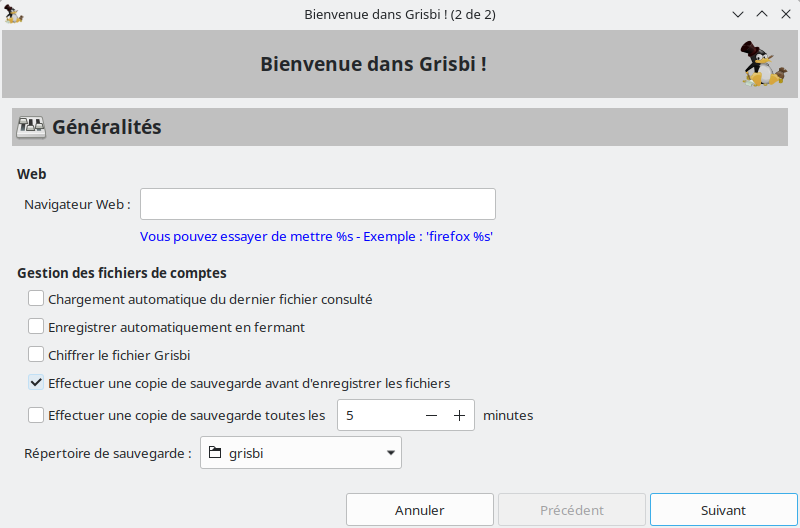
\includegraphics[width=0.9\textwidth]{image/screenshot/start_first_launch}
	\end{center}
	\caption{Configuration initiale du fichier de comptabilité.}
	\label{start_first_launch}
\end{figure}

Il est conseillé de cocher les options :

\begin{itemize}
 \item chargement automatique du dernier fichier consulté;
 \item enregistrer automatiquement en fermant;
 \item effectuer une copie de sauvegarde avant d'enregistrer les fichiers (coché par défaut).
\end{itemize}

\vspacepdf{5mm}
\textcolor{red}{\strong{Attention}}: si vous cochez l'option \menu{Chiffrer le fichier Grisbi}, la perte du mot de passe rendra votre fichier inutilisable.
\vspacepdf{5mm}

Cet assistant est suivi automatiquement par un deuxième, l'assistant de création du \indexword{fichier de comptabilité}\index{fichier de comptabilité}. Puis vient automatiquement un troisième assistant, l'assistant de création de compte, qui permet de créer le premier compte. Tout cela est décrit en détail dans la section \ref{start-newfile} ci-dessous.

À tout moment vous pouvez sortir de n'importe quel assistant par le bouton \menu{Annuler}.

Si vous ne voulez pas utiliser l'assistant premier démarrage, vous pouvez à la
place utiliser un fichier exemple (voir la section ci-dessous).


\section{Fichier exemple\label{start-example}}


Si vous voulez utiliser Grisbi immédiatement sans être obligé de rentrer tout un tas d'opérations, par exemple pour vous faire une idée des possibilités de ce logiciel, vous pouvez télécharger le fichier \file{Example\_3.0-fr.gsb} sur le site de \lang{Sourceforge.net}\footnote{\urlSourceForgeDocumentation{}} dans le dossier << \textsf{examples} >>.

% espace avant Attention ou Note  :  5mm
\vspacepdf{5mm}
\textbf{Note} : dans ce fichier exemple, les noms des tiers sont de pure invention ; seul un hasard indépendant de notre volonté peut avoir fait que ce soit celui d'une personne ou d'une entité existante.


\section{Création d'un nouveau fichier de comptabilité\label{start-newfile}}


La première fois que vous utiliserez Grisbi, vous devrez d'abord créer un \indexword{fichier
de comptabilité}\index{fichier de comptabilité} (ou fichiers de compte\textbf{S} pour Grisbi, notez le \textbf{S}). L'\gls{extension} de ce fichier sera \file{.gsb} et son nom \file{nom-de-votre-fichier.gsb}. 

Immédiatement après, il vous faudra créer au minimum un compte (bancaire, de caisse, de passif ou d'actif, décrits au chapitre \vref{accounts} \menu{Gestion des comptes}), et par la suite quelques autres comptes (comptes courants, d'épargne, de crédit, éventuellement un compte d'espèces et quelques comptes de transition) qui contiendront leurs opérations respectives. 

Pour une gestion familiale, vous n'aurez normalement qu'un seul fichier de comptabilité (que Grisbi appelle fichier de compte\textbf{S}, notez le \textbf{S}), car cela permet tous les échanges entre vos différents comptes. Si vous gérez une association, ou une autre famille sans rapport comptable avec la première, vous créerez un autre fichier de comptabilité, qui portera un autre nom \file{nom-de-votre-deuxième-fichier.gsb}. Ainsi les \indexword{entités comptables}\index{entité comptable} resteront bien séparées.

% espace avant Attention ou Note  : 5 mm
\vspacepdf{5mm} % TODO à mettre à jour au changement dans Grisbi du fichier de "comptes" par "comptabilité"
\textcolor{red}{\strong{Attention}} : pour une entité comptable donnée, il est nécessaire et important de bien distinguer LE \frquote{\indexword{fichier de comptes}\index{fichier de comptes}} et LES \frquote{\indexword{fichiers de compte}\index{fichiers de compte}} :

\begin{itemize}
	\item LE \frquote{fichier de comptes} que vous aurez créé aura pour extension \file{.gsb} et pour nom \file{nom-de-votre-fichier.gsb} ; il contient toutes les données de tous les comptes créés pour la gestion d'une entité comptable ;
	\item LES \frquote{fichiers de compte} sont des fichiers que vous pourriez être amené(e) à utiliser ou à créer pour importer ou exporter des données d'une application de comptabilité à une autre ; ces fichiers ne contiendront que les données d'un seul compte (courant ou autre) à la fois ; ils auront des extensions différentes (\file{.ofx}, \file{.csv} ou \file{.qif}) suivant leur contenu ; pour plus de détails, voir le chapitre \vref{move}, \menu{Export et import de comptes}.
\end{itemize}
% espace après Attention ou Note  : 5 mm
\vspacepdf{5mm}

Autrement dit, l'ensemble des comptes de votre foyer est enregistré dans un fichier de comptabilité, et l'ensemble des comptes de votre association l'est dans un autre fichier de comptabilité; et un compte dans Grisbi peut correspondre à un fichier de compte, mais seulement lorsqu'on parle d'importation ou d'exportation de données.

% espace pour changement de thème
\vspacepdf{5mm}
Le déroulement général de la procédure de création d'un fichier de comptabilité est le suivant : cliquez sur le menu \menu{Fichier > Nouveau fichier de comptabilité} ; l'assistant de création de fichier de comptabilité s'ouvre, qui comprend six étapes. À la sixième étape, l'assistant vous propose :

\begin{itemize}
	\item  soit de créer un nouveau compte, et il enchaîne sur l'assistant de création de compte, qui comprend lui-même cinq étapes, pour créer le premier compte (car il est indispensable de disposer d'au moins un compte) ;
	\item soit d'utiliser des données déjà existantes, et il enchaîne alors sur l'assistant d'importation des opérations, qui comprend aussi cinq étapes, pour importer des opérations de comptes existants.
\end{itemize}

Après la création de ce premier compte ou l'importation d'opérations de comptes existants, si vous voulez créer d'autres comptes, vous retournerez à la fin de la procédure de création du fichier de comptes, ce qui vous renverra dans les deux cas vers la création d'un nouveau compte.

% espace pour changement de thème
\vspacepdf{5mm}
Pour créer votre fichier de comptabilité, cliquez sur le menu \menu{Fichier > Nouveau fichier de comptabilité}, la procédure détaillée est la suivante:

\begin{enumerate}
	\item Fenêtre d'accueil : validez par le bouton \menu{Suivant} (étape 1/6) :
	\item Configuration
%		\ifIllustration
 générale (étape 2/6)%\refimage{start_file_create-img}
 :

%		\else générale :
%		\fi

%		\ifIllustration
		% image centrée
		\begin{figure}[htbp]
		\begin{center}
		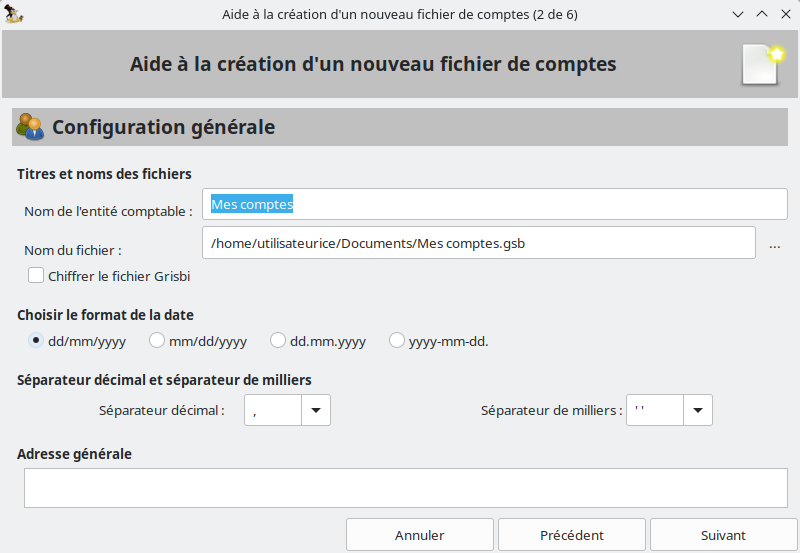
\includegraphics[width=0.9\textwidth]{image/screenshot/start_file_create}
		\end{center}
		\caption{Configuration générale du fichier de comptabilité}
		\label{start-file-create}
		\end{figure}
		% image centrée
%		\fi
		
		\begin{enumerate} 
		 	\item choisissez le nom de l'entité comptable dont vous gérez la comptabilité, par exemple \frquote{Ma comptabilité}, qui pourra être choisi comme titre de la page d'accueil de l'application Grisbi,
			\item saisissez le nom du fichier de comptes avec son arborescence complète ; Grisbi vous propose par défaut le même nom que celui de l'entité comptable, mais vous pouvez le modifier,
			\item cochez la case \menu{Chiffrer le fichier Grisbi} si vous voulez \gls{chiffrer} le fichier de comptes,
			
			\vspacepdf{2mm}
			\textcolor{red}{\strong{Attention}}: si vous cochez l'option \menu{Chiffrer le fichier Grisbi}, la perte du mot de passe rendra votre fichier inaccessible.
			\vspacepdf{2mm}
			
			\item sélectionnez le \indexword{format de la date}\index{format de date} avec l'un des quatre boutons :
			\begin{addmargin}{-0.2cm}
				\begin{itemize}	
				\item "dd/mm/yyyy" pour "jour/mois/année",
				\item "mm/dd/yyyy" pour "mois/jour/année",
				\item "dd.mm.yyyy" pour "jour.mois.année",
				\item "yyyy-mm-dd" pour "année-mois-jour",
				\end{itemize}
			\end{addmargin}
			\item choisissez le \indexword{séparateur}\index{séparateur} décimal et celui des milliers dans les listes déroulantes,
			 \item renseignez l'adresse (facultatif),
			 \item  validez par le bouton \menu{Suivant} ;
		\end{enumerate}
		
	\item Sélection de la \indexword{devise}\index{devise} de base (étape 3/6):
		\begin{enumerate} 
		 	\item cliquez sur la devise choisie dans la liste,
			\item cochez la case \menu{Afficher les devises obsolètes} si vous voulez aussi afficher d'anciennes devises,
			\item validez par le bouton \menu{Suivant};
		\end{enumerate}

	\item sélection des \indexword{types de catégories}\index{catégories !types} utilisées (étape 4/6):
	
	\begin{figure}[htbp]
	\begin{center}
		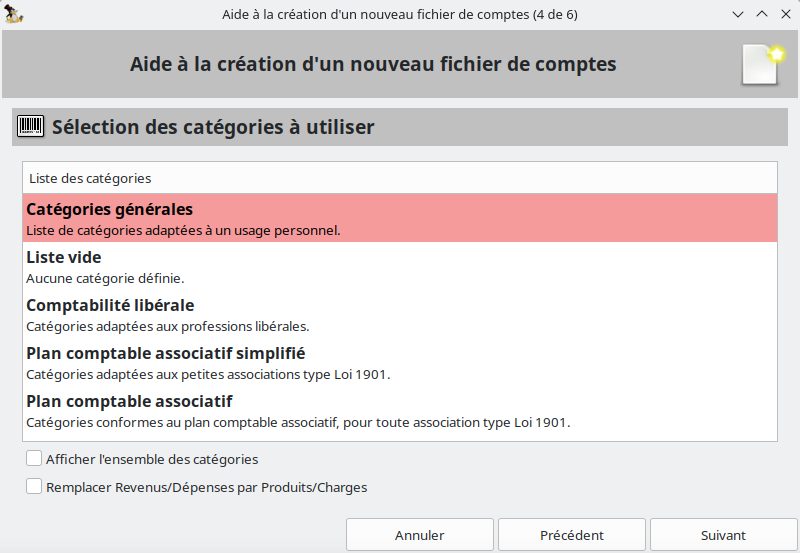
\includegraphics[width=0.9\textwidth]{image/screenshot/start_category_select}
	\end{center}
	\caption{Sélection des catégories à utiliser}
	\label{start_category_select}
	\end{figure}
		
		\begin{enumerate} 
		 	\item cliquez sur la catégorie choisie dans la liste ci-dessus:
%		 	\begin{itemize}
%		 		\item\menu{Catégories générales},
%		 		\item \menu{Liste vide},
%		 		\item\menu{Comptabilité libérale},
%		 		\item\menu{Plan comptable associatif simplifié}
%		 		\item\menu{Plan comptable associatif},
%		 	\end{itemize}
			\item cochez la case \menu{Afficher l'ensemble des catégories} si vous voulez aussi afficher d'autres catégories libellées en anglais,
			\item validez par le bouton \menu{Suivant} ;
		\end{enumerate}		

	\item Définition des \indexword{banques}\index{banques !définition} détenant vos comptes (étape 5/6):
		\begin{enumerate} 
		 	\item cliquez sur  \menu{Ajouter} pour définir une banque ; renseignez les détails de la banque (nom, code banque, etc.), puis validez par le bouton \menu{Ajouter} pour valider la banque,
			\item sélectionnez une banque dans la liste et validez par le bouton \menu{Enlever} pour supprimer une banque, puis confirmez dans la fenêtre qui s'ouvre,
			\item répétez les actions a et b autant de fois que nécessaire,
			\item  validez par le bouton \menu{Suivant} pour passer à l'étape suivante, \menu{Création d'un nouveau compte} ;
		\end{enumerate}		 	

	\item Configuration terminée (étape 6/6):\par
	La configuration du fichier de comptabilité est terminée, et la fenêtre ci-dessous vous propose de choisir l'une des deux méthodes de création de votre premier
%\ifIllustration
compte:%\refimage{start-account-choice-img} :
%\else compte :
%\fi
\vspace{5mm}
%\ifIllustration
% image centrée
\begin{figure}[htbp]
\begin{center}
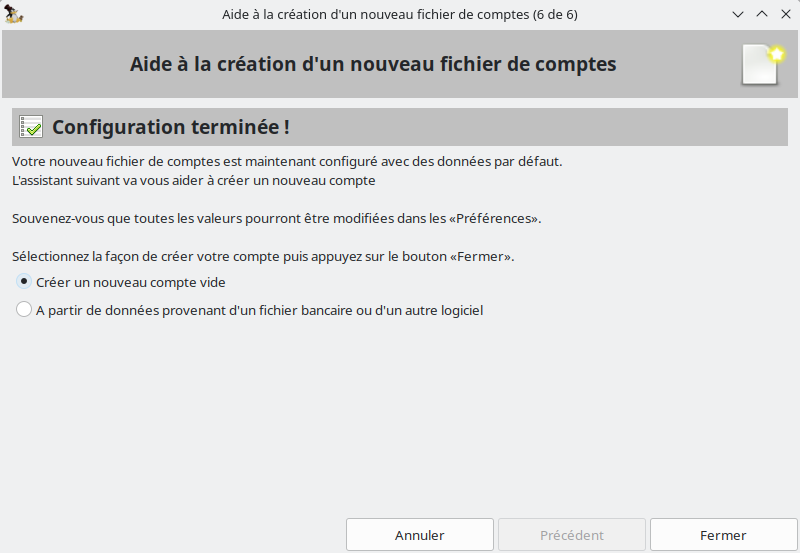
\includegraphics[width=0.9\textwidth]{image/screenshot/start_account_choice}
\end{center}
\caption{Choix du premier compte}
\label{start_account_choice}
\end{figure}
% image centrée
%\fi

		\begin{itemize}
			\item \menu{Créer un nouveau compte vide} : si vous cochez cette ligne, puis si vous validez par le bouton \menu{Fermer}, cette fenêtre se ferme et l'assistant de création de nouveau compte démarre. Reportez-vous à la section \vref{accounts-new}, \menu{Création d'un nouveau compte}, qui décrit entièrement cette procédure, puis revenez à cette page ;

			\item \menu{À partir de données provenant d'un fichier bancaire ou d'un autre logiciel} : si vous cochez cette ligne, puis si vous validez par le bouton \menu{Fermer}, cette fenêtre se ferme et l'assistant d'importation des données d'un fichier de compte par Grisbi démarre. Reportez-vous à la section \vref{move-import-importinit}, \menu{Import de fichiers de compte d'un autre logiciel dans Grisbi}, qui décrit entièrement cette procédure, puis revenez à cette page.
		\end{itemize}
\end{enumerate}

% étiquette du paragraphe suivant, pour que les liens hypertexte dans account.tex et QIF.tex  arrivent bien dessus
\label{start-newfile-end}

\textit{\textbf{D'une manière ou d'une autre}}, vous venez donc de créer votre fichier de comptabilité, ainsi que le premier compte de ce fichier. 

%espace pour changement de thème
\vspacepdf{5mm}
Si vous voulez créer maintenant d'autres comptes, sélectionnez le menu \menu{Édition - Nouveau compte} pour créer un autre compte (voir la section \vref{accounts-new}, \menu{Création d'un nouveau compte}).

%espace pour changement de thème
\vspacepdf{5mm}
Sinon, vous pouvez commencer à utiliser le compte que vous venez de créer ou celui dont vous venez d'importer les données.

% espace avant Attention ou Note  : 5 mm
\vspacepdf{5mm}
\textcolor{red}{\strong{Attention}} : d'une manière générale, il est déconseillé d'avoir des accents ou des espaces dans les noms des répertoires et fichiers utilisés par Grisbi. Si c'est le cas, renommez-les maintenant. Par exemple, les espaces peuvent être remplacées par des tirets bas (\_).

% saut de page pour titre solidaire
%\newpage


\section{Enregistrement de votre fichier de comptabilité\label{start-save}}


Vos opérations ne sont pas écrites au fur et à mesure de leur saisie comme 
elles peuvent l'être dans d'autres logiciels; vous devez donc enregistrer votre fichier de comptabilité avant de quitter. N'ayez crainte, Grisbi vous prévient si vous ne l'avez pas fait. 

Vous pouvez configurer les options d'enregistrement du fichier de comptabilité dans le menu \menu{Édition - Préférences}, voir le paragraphe \vref{setup-general-files-manage}, \menu{Gestion des fichiers de comptes}.


\section{Import à partir d'un autre logiciel de comptabilité personnelle}

Voir la section \vref{move-import-importinit} pour importer des fichiers de compte d'un autre logiciel dans Grisbi.  Pour le moment, Grisbi supporte les formats \gls{Gnucash}, \gls{OFX}, \GLS{CSV} et \GLS{QIF}.


				% TODO: update screenshots and text "start", remove % when finished
%\cleardoubleemptypage

%%%%%%%%%%%%%%%%%%%%%%%%%%%%%%%%%%%%%%%%%%%%%%%%%%%%%%%%%%%%%%%%%%
% Contents: The home chapter
% $Id: grisbi-manuel-home.tex, v 0.4 2002/10/27 Daniel Cartron
% $Id: grisbi-manuel-home.tex, v 0.5.0 2004/06/01 Loic Breilloux
% $Id: grisbi-manuel-home.tex, v 0.6.0 2011/11/17 Jean-Luc Duflot
% some of its content was in menus chapter:
% $Id: grisbi-manuel-menus.tex, v 0.5.0 2004/06/01 Loic Breilloux
% $Id: grisbi-manuel-home.tex, v 0.8.9 2012/04/27 Jean-Luc Duflot
% $Id: grisbi-manuel-home.tex, v 1.0 2014/02/12 Jean-Luc Duflot
%%%%%%%%%%%%%%%%%%%%%%%%%%%%%%%%%%%%%%%%%%%%%%%%%%%%%%%%%%%%%%%%%

\chapter{Entrée dans Grisbi\label{entrance}}

\section{Sélection d'un fichier\label{select-file}}

\vspacepdf{5mm}			% vertical space = 5 mm

Au lancement de l'application, Grisbi affiche la page qui vous permet de démarrer de différentes manières.

\vspacepdf{5mm}			% espace : 5 mm

Vous pouvez afficher la fenêtre de Grisbi en \indexword{plein écran}\index{affichage!plein écran}\index{plein écran!affichage} par la touche de fonction \key{F11}, et revenir en arrière par la même touche.			% "!" separates the term from the subterm of the index entry

\vspacepdf{5mm}			% espace : 5 mm

%\ifIllustration
\begin{figure}[htbp]			% h=here, t=top, b=bottom, p=page of float to force the figure here, not in a next page.
	\begin{center}					% image centrée
		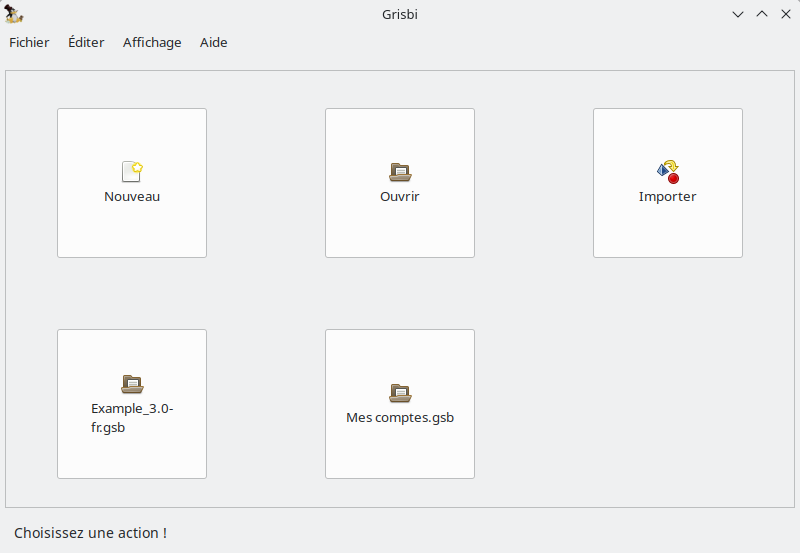
\includegraphics[width=0.95\textwidth]{image/screenshot/start_grisbi}		% width=95% as wide as the current text
	\end{center}
	\caption{Fenêtre de démarrage}			% sous-titre/subtitle
	\label{start_grisbi}					% figure's ref., use for link in text with \refimage{}
\end{figure}
%\fi

\vspacepdf{3mm}			% espace : 5 mm

En plus de la barre de menu, cette fenêtre affiche plusieurs pavés:

\begin{itemize}
	\item le pavé Nouveau, pour lancer l'assistant \frquote{Aide à la création d'un nouveau fichier de comptes};
	\item le pavé Ouvrir, pour afficher un gestionnaire de fichier avec lequel vous pourrez chercher un fichier de comptes existant dans votre ordinateur;
	\item le pavé Importer, pour lancer l'assistant \frquote{Importation des opérations par Grisbi};
	\item un ou plusieurs autres pavés, portant le nom de fichiers de comptes que Grisbi a déjà utilisés.
\end{itemize}


\textbf{Note}: les pavés portant les noms des fichiers de comptes que Grisbi a déjà utilisés ne sont présents que si ces fichiers existent; si vous voulez les enlever de cette page d'entrée, déplacez-les dans un autre répertoire, ou supprimez-les.

\vspacepdf{5mm}			% espace : 5 mm

En bas de page, un bandeau vous appelle à choisir une action en sélectionnant l'un de ces pavés.

\vspacepdf{5mm}			% espace : 5 mm

Si vous voulez juste découvrir le logiciel Grisbi pour avoir un aperçu de son aspect et de ses possibilités, vous pouvez à la place utiliser un fichier exemple comme celui présent sur le site de \lang{Sourceforge.net}\footnote{\urlSourceForgeDocumentation{}} dans le dossier \frquote{\textsf{examples}}.		% (voir la section \vref{new-example}).

\vspacepdf{5mm}			% espace : 5 mm

\textbf{Note}: en cliquant simplement sur le fichier exemple téléchargé, Grisbi affichera directement la fenêtre d'accueil\refimage{home} sans passer par la fenêtre de démarrage.


\section{Accueil\label{home}}

\vspacepdf{5mm}

En ouvrant un fichier de comptes, Grisbi affiche sa page d'accueil\refimage{home-img}.
C'est la page de démarrage du programme; on peut y accéder à tout moment en cliquant sur l'onglet \menu{Comptes}. 

\vspacepdf{3mm}

\begin{figure}[htbp]			% h=here, t=top, b=bottom, p=page of float to force the figure here, not in a next page.
\begin{center}
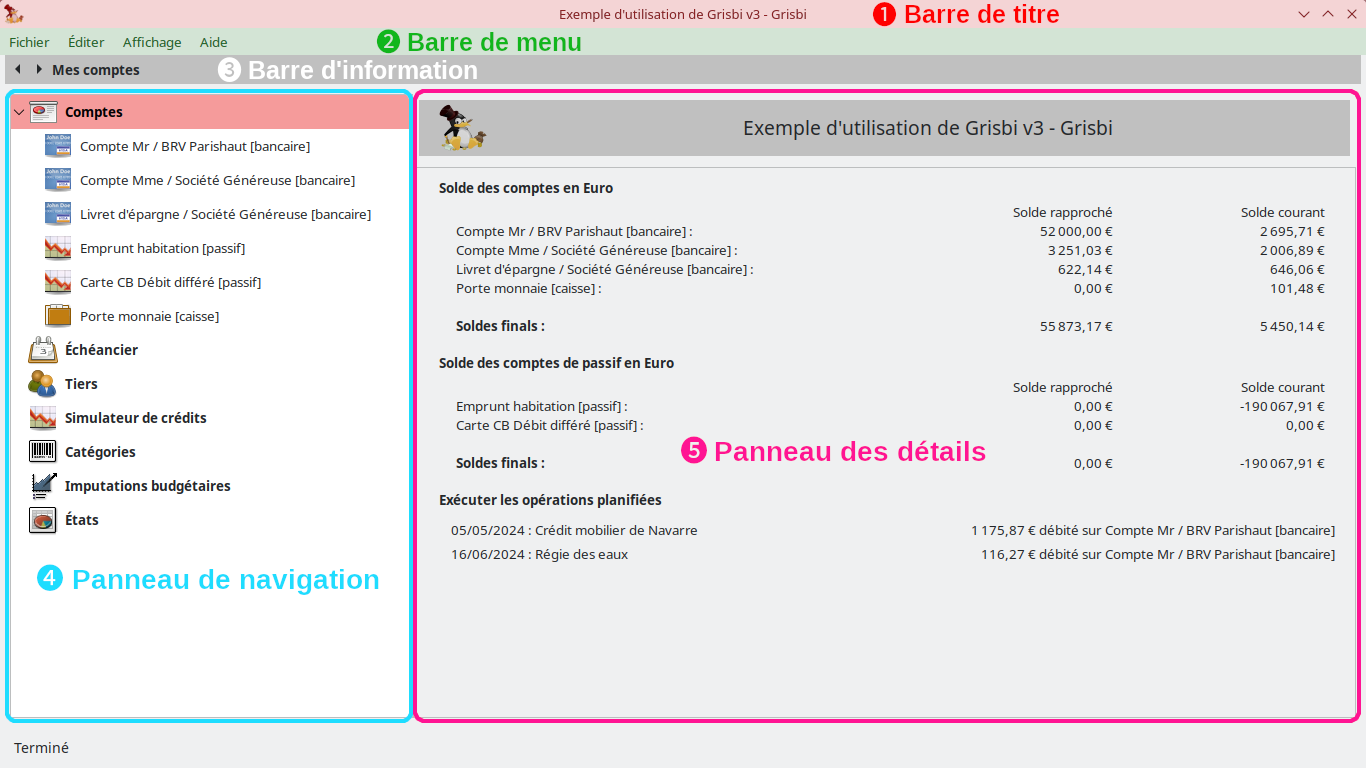
\includegraphics[width=1\textwidth]{image/screenshot/home}
\end{center}
\caption{Page d'accueil}		% sous-titre/subtitle
\label{home-img}
\end{figure}

\vspacepdf{3mm}

Grisbi affiche toutes ses pages de la même manière: comme n'importe quel logiciel, il affiche:% une barre de titre, une barre de menus qui donne accès à la plupart des fonctionnalités importantes de Grisbi, et aussi trois zones:

\begin{itemize}%[\large \textcircled{\small 2}]
	\item[\large\textcircled{\small 1}] une barre de titre;
	\item[\large\textcircled{\small 2}] une barre de menus qui donne accès à la plupart des fonctionnalités importantes de Grisbi;
\end{itemize}
et aussi trois zones qui sont spécifiques à Grisbi:
\begin{itemize}%[3,4,5]
	\item[\large\textcircled{\small 3}] la barre d'information, sous la barre de menus;
	\item[\large\textcircled{\small 4}] le panneau de navigation;
	\item[\large\textcircled{\small 5}] le panneau des détails
\end{itemize}

%Les zones 3, 4 et 5 sont spécifiques à Grisbi%, sont encadrées de couleurs dans la figure pour bien les identifier\refimage{home}.


\section{Barre d'information\label{home-synthesis}}


La barre d'information affiche le nom de l'onglet courant affiché, et peut afficher, complètement à droite, certains soldes en rapport avec ce qui est sélectionné dans le pavé des détails.

% espace pour changement de thème
\vspacepdf{5mm}
Elle permet, en cliquant successivement sur l'un des deux petits triangles à sa gauche, de sélectionner l'un des onglets affichés dans le panneau de navigation: \menu{Comptes}, \menu{Échéancier}, \menu{Tiers}, \menu{Simulateur de crédits}, \menu{Catégories}, \menu{Imputations budgétaires} et \menu{États}, et aussi l'un des sous-onglets des onglets \menu{Comptes} et \menu{États} s'ils sont déroulés dans le panneau de navigation.

\vspacepdf{5mm}
% Pas de commande au clavier pour cette fonction
\textbf{Note}: ces triangles peuvent être remplacés, en fonction du thème de l'environnement de bureau ou du gestionnaire de fenêtres que vous utilisez, par d'autres caractères tels que +, -, >, <, etc.

% espace pour changement de thème
\vspacepdf{3mm}
Le contenu de la sélection s'affiche dans le pavé des détails.

% espace pour changement de thème
\vspacepdf{3mm}
Ces fonctionnalités peuvent être utilisées à la place de celles du panneau de navigation lorsque sa largeur est réduite à zéro et que l'on n'y a pas accès directement.


\section{Panneau de navigation\label{home-accounting}}


Le panneau de navigation affiche en caractères gras la liste des onglets: \menu{Comptes}, \menu{Échéancier}, \menu{Tiers}, \menu{Simulateur de crédits}, \menu{Catégories}, \menu{Imputations budgétaires} et \menu{États}. En cliquant sur le petit triangle noir à gauche des onglets \menu{Comptes} ou \menu{États}, on peut dérouler ou enrouler la liste de leurs sous-onglets. Vous pouvez changer l'ordre des onglets et des sous-onglets en cliquant sur l'un d'eux et en le déplaçant plus haut ou plus bas dans la liste.

\vspacepdf{3mm}

\textbf{Note}: ces triangles peuvent être remplacés, en fonction du thème de l'environnement de bureau ou du gestionnaire de fenêtres que vous utilisez, par d'autres caractères tels que +, -, >, <, etc.

% espace pour changement de thème
\vspacepdf{5mm}
Vous pouvez sélectionner un de ces onglets ou sous-onglets en cliquant sur son nom. Vous pouvez aussi déplacer la sélection dans cette liste d'onglets et de sous-onglets avec les touches du clavier \key{Flèche Haut}, \key{Flèche Bas}, \key{Pg. Préc} ou \key{Pg. Suiv}, ou avec la molette de la souris. 

% espace pour changement de thème
\vspacepdf{5mm}
Le contenu de la sélection s'affiche dans le pavé des détails. 

% espace pour changement de thème
\vspacepdf{5mm}
On peut réduire ou agrandir la largeur du panneau de navigation en cliquant sur la fine barre verticale entre ce panneau et le pavé des détails, et en la déplaçant. Si la largeur du panneau a été réduite à zéro, ou agrandie au maximum de la largeur de la fenêtre de Grisbi, il faut retrouver cette barre, respectivement complètement à gauche ou à droite de la fenêtre, et la faire glisser à la place désirée. 

% espace pour changement de thème
\vspacepdf{5mm}
Des \indexword{menus contextuels}\index{menu contextuel}, accessibles par un clic-droit de souris, sont disponibles sur les éléments de ce panneau et proposent les fonctions suivantes:

\begin{itemize}
	 \item sur \menu{Comptes}:
		\begin{itemize}
			 \item \menu{Nouveau compte};
		\end{itemize}
	 \item sur un compte quelconque: 
		\begin{itemize}
			 \item \menu{Nouveau compte},
			 \item \menu{Supprimer ce compte};
		\end{itemize}
	 \item sur \menu{Tiers}:
		\begin{itemize}
			 \item \menu{Nouveau tiers},
			 \item \menu{Supprimer le tiers sélectionné},
			 \item \menu{Éditer le tiers sélectionné},
			 \item \menu{Gérer les tiers},
			 \item \menu{Supprimer les tiers inutilisés};
		\end{itemize}
	 \item sur \menu{Catégories}: 
		\begin{itemize}
			 \item \menu{Nouvelle catégorie},
			 \item \menu{Supprimer la catégorie sélectionnée},
			 \item \menu{Editer la catégorie sélectionnée},
			 \item \menu{Importer un fichier de catégories (.csgb)},
			 \item \menu{Exporter la liste des catégories (.csgb)};
		\end{itemize}
	 \item sur \menu{Imputations budgétaires}:
		\begin{itemize}
			 \item \menu{Nouvelle imputation budgétaire},
			 \item \menu{Supprimer l'imputation sélectionnée},
			 \item \menu{Editer l'imputation sélectionnée},
			 \item \menu{Importer un fichier d'imputations budgétaires (.isgb)},
			 \item \menu{Exporter la liste des imputations budgétaires (.isgb)};
		\end{itemize}
	 \item sur \menu{État}: \menu{Nouvel état};
	 \item sur un état quelconque: 
		\begin{itemize}
			 \item \menu{Nouvel état},
			 \item \menu{Supprimer cet état}.
		\end{itemize}
\end{itemize}

% saut de page pour titre solidaire
\newpage


\section{Pavé des détails\label{home-details}}


Le pavé des détails affiche tous les détails sur les onglets ou sous-onglets sélectionnés par la barre d'information ou le panneau de navigation. C'est la zone de travail principale de Grisbi.

On peut réduire ou agrandir sa largeur en cliquant sur la fine barre verticale entre ce pavé et le panneau de navigation, et en la déplaçant. Si la largeur du pavé a été réduite à zéro ou agrandie au maximum de la largeur de la fenêtre de Grisbi, il faut retrouver cette barre, respectivement complètement à droite ou à gauche de la fenêtre, et la faire glisser à la place désirée. 
 
% TODO: LA SUITE
 
\subsection{Affichage de la page d'accueil\label{home-details-homepage}}

Pour afficher la page d'accueil, sélectionnez l'onglet \menu{Comptes}; le pavé des détails affiche, de haut en bas:

\begin{itemize}
	 \item dans un pavé sur fond gris, l'icône \menu{Grisbi} à gauche, et à droite un \indexword{titre}\index{affichage!titre}\index{titre!page d'accueil} qui permet d'identifier sur quelle comptabilité vous travaillez actuellement, sous la forme \frquote{libellé - Grisbi}; vous pouvez définir ce libellé, parmi trois possibilités, dans le menu \menu{Édition - Préférences} (voir le paragraphe \vref{setup-display-addresses-titles}, \menu{Titres}):
		\begin{itemize}
			 \item l'\menu{Entité comptable}: c'est le nom du domaine de comptabilité sur lequel vous travaillez, par exemple \frquote{Ma comptabilité} ou \frquote{Association}, et que vous avez saisi à la création du fichier de comptes; vous pouvez le modifier ici dans le champ \menu{Nom de l'entité comptable}; cela peut être utile si vous gérez plusieurs \indexword{entités comptables}\index{entité comptable}, 
			 \item le \menu{Titulaire du compte}: c'est le nom du titulaire (ou du propriétaire) du dernier compte consulté; si le titulaire n'est pas renseigné dans les propriétés du compte, Grisbi affiche le nom de ce compte,
			 \item le \menu{Nom du fichier de comptes}: c'est le nom du fichier dans le répertoire courant, sous la forme \file{nom\_de\_\_votre\_fichier.gsb}, et c'est le choix par défaut;
		\end{itemize}
	 \item pour chaque devise séparément, pour tous les comptes et \indexword{groupes de comptes}\index{groupe de comptes}, sous les libellés \menu{Solde rapproché} et \menu{Solde courant}:
		\begin{itemize}
			 \item le solde des comptes bancaires et comptes de caisse, le solde partiel des groupes de comptes et leur solde final,
% saut de ligne pour indentation correcte de la note dans la liste

			 \textbf{Note}: vous pouvez ajuster l'ordre d'affichage des soldes partiels des groupes de comptes (voir le paragraphe \vref{setup-general-home-partBalance}, \menu{Soldes partiels de la liste des comptes}).			 
			 \item le solde des comptes de passif et leur solde final,
			 \item le solde des comptes d'actif et leur solde final;
		\end{itemize}
	\item les \indexword{alertes des opérations planifiées}\index{alerte!opération planifiée} à échéance ou clôturées, avec leurs date, libellé et montant, selon les choix faits dans le menu \menu{Édition - Préférences} (voir la section \vref{setup-general-planned}, \menu{Échéancier});
	\item la liste des comptes dont le solde est passé sous le \menu{Solde minimal autorisé};
	\item la liste des comptes dont le solde est passé sous le \menu{Solde minimal voulu}.
\end{itemize}

% espace avant Attention ou Note: 5 mm
\vspacepdf{5mm}

\textbf{Note}: pour les définitions du \menu{Solde minimal autorisé} et du \menu{Solde minimal voulu}, voir la section \vref{accounts-properties}, \menu{Propriétés d'un compte}.

% espace pour changement de thème
\vspacepdf{5mm}
Les libellés des comptes s'affichent en \textcolor{black}{noir}; au passage du pointeur de la souris sur la ligne de l'un d'eux, cette couleur passe au \textcolor{gray}{gris}.
Un solde supérieur au \menu{Solde minimal voulu} s'affiche en \textcolor{teal}{vert foncé}; au passage du pointeur sur sa ligne, cette couleur passe au \textcolor{lime}{vert clair}.
Un solde inférieur au \menu{Solde minimal voulu} et supérieur au \menu{Solde minimal autorisé} s'affiche en \textcolor{orange}{orange}; au passage du pointeur sur sa ligne, cette couleur passe à l'\textcolor{orange}{orange clair}.
Un solde inférieur au \menu{Solde minimal autorisé} s'affiche en \textcolor{red}{rouge}; au passage du pointeur sur sa ligne, cette couleur passe au \textcolor{red}{rouge clair}.

Au passage du pointeur de la souris sur la ligne d'un compte, tout changement de couleur indique que si l'on clique (droit ou gauche) avec la souris, ce compte s'affiche, comme s'il avait été sélectionné avec la barre d'information ou le panneau de navigation; il affiche alors la page qui contient la ligne d'opération affichant ce solde.

Un solde partiel, qui correspond à un groupe de comptes, s'affiche en \textcolor{black}{noir}. S'il est négatif, il peut s'afficher en \textcolor{red}{rouge foncé}, mais seulement si cela a été configuré ainsi (voir le paragraphe \vref{setup-general-home-partBalance}, \menu{Soldes partiels de la liste des comptes}). Une ligne de solde partiel ne change pas de couleur au passage du pointeur de la souris dessus, car on ne peut pas afficher les opérations d'un groupe de comptes.

% espace pour changement de thème
\vspacepdf{5mm}
Vous pouvez configurer certains aspects de l'affichage de cette page d'accueil dans le menu \menu{Édition - Préférences} ou dans l'onglet \menu{Propriétés} de chaque compte:
\begin{itemize}
	 \item \menu{\indexword{Polices}\index{polices}, \indexword{logo}\index{logo} et \indexword{couleurs}\index{couleurs}}: section \vref{setup-display-logo};
	 \item \menu{Titres}: section \vref{setup-display-addresses-titles};
	 \item \menu{Calcul des soldes}: paragraphe \vref{setup-general-home-balance};
	 \item \menu{Soldes partiels de la liste des comptes}: paragraphe \vref{setup-general-home-partBalance};
	 \item \menu{Alertes de l'échéancier}: section \vref{setup-general-planned};
	 \item comptes sous le \menu{\indexword{Solde minimal autorisé}}\index{solde!minimal autorisé}: section \vref{accounts-properties};
	 \item comptes sous le \menu{\indexword{Solde minimal voulu}}\index{solde!minimal voulu}: section \vref{accounts-properties}.
\end{itemize}

En particulier, si vous trouvez une erreur d’orthographe dans cette page, vous pourrez la corriger: voir le paragraphe \vref{setup-general-home-final}, \menu{Pluriel de final}!

%\ifIllustration
% saut de page pour paragraphe solidaire
%\newpage
%\fi

\section{Barre de menus\label{home-menus}}


Comme dans de nombreuses applications graphiques, la plupart des fonctionnalités importantes de Grisbi sont accessibles au moyen des menus de la \indexword{barre de menus}\index{barre de menus}. Nous détaillons ici leurs fonctionnalités.


\subsection{Menu \menu{Fichier}\label{home-menus-file}}

Ce menu comprend les fonctions suivantes:

\begin{itemize}
	\item \menu{Nouveau fichier de comptes}: crée un nouveau fichier de comptes; le fichier courant est donc fermé et un nouveau fichier vide est créé avec un compte vide (raccourci-clavier \key{Ctrl}\key{N}), voir la section \vref{start-newfile}; à ne pas confondre avec la création d'un nouveau compte;
	\item \menu{Ouvrir}: ouvre un fichier de comptes (raccourci-clavier \key{Ctrl}\key{O});
	\item \menu{Derniers fichiers}: affiche la liste des n derniers fichiers ouverts avec Grisbi (seulement s'il y en a eu plusieurs); ce nombre est configurable dans le menu \menu{Edition - Préférences}, voir la section \vref{setup-general-files-manage}, \menu{Gestion des fichiers de compte};
	\item \menu{Enregistrer} enregistre le fichier de comptes en cours (raccourci-clavier \key{Ctrl}\key{S});
	\item \menu{Enregistrer sous}: ouvre un gestionnaire de fichiers pour enregistrer le fichier de comptes en cours avec le nom et à l'emplacement de 	votre choix; Grisbi vous propose par défaut le répertoire courant, le nom du fichier de comptes en cours, avec l'extension \file{.gsb};
	\item \menu{Importer un fichier}: démarre l'assistant d'importation de fichiers d'un autre logiciel; voir la section \vref{move-import-importinit};
	\item \menu{Exporter vers un fichier QIF/CSV}: démarre l'assistant d'exportation de fichiers de compte; voir la section \vref{move-export};	
	\item \menu{Créer une archive}: démarre l'assistant de création d'archive; voir la section \vref{datamanagement-history-new};	
	\item \menu{Exporter une archive vers un fichier GSB/QIF/CSV}: démarre l'assistant d'exportation d'archive; voir la section \vref{datamanagement-history-export};
	\item \menu{Déboguer le fichier de compte}: démarre l'assistant de 	débogage de ce fichier, qui va vous aider à chercher des incohérences dans votre fichier de comptes; voir la section \vref{maintenance-file-debug};
	\item \menu{Rendre anonyme le fichier de comptes}: démarre l'assistant qui produit une copie anonymée de votre fichier de comptes; ce fichier pourra être joint à un rapport de bogue; voir la section \vref{maintenance-file-anonymous};	
	\item \menu{Rendre anonyme le fichier QIF}: démarre l'assistant qui produit une copie anonymée de ce fichier; ce fichier pourra être joint à un rapport de bogue; voir la section \vref{maintenance-QIF-anonymous};	
	\item \menu{Mode de débogage}: met Grisbi en mode de débogage, qui crée un fichier-journal des évènements; voir la section \vref{maintenance-debug-mode}; 	
	\item \menu{Fermer}: ferme le fichier de comptes en cours; Grisbi vous propose de l'enregistrer si ce n'est déjà fait (raccourci-clavier \key{Ctrl}\key{W});
	\item \menu{Quitter}: ferme Grisbi; Grisbi vous propose auparavant d'enregistrer le fichier de comptes, si ce n'est pas déjà fait (raccourci-clavier \key{Ctrl}\key{Q}).
\end{itemize}


\subsection{Menu \menu{Édition}\label{home-menus-edit}}

Ce menu comprend les fonctions suivantes:

\begin{itemize}
	\item \menu{Editer l'opération}: voir la section \vref{transactions-modify}, \menu{Modification d'une opération};
	\item \menu{Nouvelle opération}: voir la section \vref{transactions-new}, \menu{Saisie d'une nouvelle opération};
	\item \menu{Supprimer une opération}: voir la section \vref{transactions-delete}, \menu{Suppression d'une opération};
	\item \menu{Utiliser l'opération sélectionnée comme modèle}: voir la section \vref{transactions-model}, \menu{Opération sélectionnée comme modèle};
	\item \menu{Cloner l'opération}: voir la section \vref{transactions-duplicate}, \menu{Clonage d'une opération};
	\item \menu{Convertir en opération planifiée}: voir la section \vref{transactions-schedule}, \menu{Conversion d'une opération en opération planifiée};
	\item \menu{Déplacer l'opération vers un autre compte}: voir la section \vref{transactions-move}, \menu{Déplacement d'une opération vers un autre compte};
	\item \menu{Nouveau compte}: voir la section \vref{accounts-new}, \menu{Création d'un nouveau compte};
	\item \menu{Supprimer le compte courant}: voir la section \vref{accounts-delete}, \menu{Suppression d'un compte};
	\item \menu{Préférences}: permet de configurer Grisbi; voir le chapitre \vref{setup}, \menu{Configuration de Grisbi}.
\end{itemize}


\subsection{Menu \menu{Affichage}\label{home-menus-display}}

Ce menu comprend les fonctions suivantes; 

\begin{itemize}
	 \item \menu{Montrer le formulaire de saisie d'opérations}; 
	 \item \menu{Montrer les opérations rapprochées} (raccourci-clavier \key{Alt}\key{R});
	 \item \menu{Montrer les lignes d'archives} (raccourci-clavier \key{Altl}\key{L});
	 \item \menu{Montrer les \indexword{comptes clos}}\index{compte!clos};
	 \item \menu{Montrer une ligne par opération};
	 \item \menu{Montrer deux lignes par opération};
	 \item \menu{Montrer trois lignes par opération};
	 \item \menu{Montrer quatre lignes par opération};
	 \item \menu{Réinitialiser la largeur des colonnes}; permet de remettre les colonnes des listes d'opérations à leur largeur d'origine.
\end{itemize}


\subsection{Menu \menu{Aide}\label{home-menus-help}}

La plupart des choix de ce menu donnent accès à des sites Web. Pour que ces accès fonctionnent, il faut avoir indiqué à Grisbi le logiciel de navigation (ou navigateur) que vous souhaitez utiliser, dans le menu \menu{Édition - Préférences} (voir la section \vref{setup-general-programs}, \menu{Programmes}). Le menu \menu{Aide} comprend les choix suivants;

\begin{itemize}
	\item \menu{Manuel}; ouvre votre navigateur à la page \frquote{Manuel de l'Utilisateur de Grisbi} (raccourci-clavier \key{Ctrl}\key{H});
	\item \menu{Démarrage rapide}; ouvre votre navigateur à la page \frquote{Démarrage Rapide de Grisbi};
	\item \menu{Traduction}; ouvre votre navigateur à la page \frquote{Traduire Grisbi}, pour vous inviter à nous aider à l'élargissement de 	l'internationalisation de Grisbi;
	\item \menu{À propos de Grisbi}; affiche la boîte d'information sur l'application; vous y trouverez des détails sur la version, le lien vers le site de Grisbi, les remerciements (contributeurs au projet) et la licence d'utilisation;
	\item \menu{Site Web de Grisbi}; ouvre votre navigateur à la page du site de \lang{Grisbi}\footnote{\urlGrisbi{}};
	\item \menu{Signaler une anomalie}; ouvre votre navigateur à la page du \lang{traqueur de bogues de Grisbi}\footnote{\urlBugTracker{}} pour vous permettre de signaler un bogue que vous auriez découvert. Vous pouvez également suivre sur cette page l'évolution des corrections apportées aux bogues signalés;
	\item \menu{Astuce du jour}; ouvre une boîte de dialogue qui affiche une astuce d'utilisation, différente à chaque démarrage de Grisbi; vous pouvez y 	afficher successivement toutes les astuces, et choisir ou non l'affichage de 	l'astuce du jour au démarrage de Grisbi. Pour supprimer ou réactiver l'astuce du 	jour, voir le paragraphe \vref{setup-display-messages-trick}, \menu{Astuce du jour}.
\end{itemize}


\section{Raccourcis-clavier\label{home-shortcuts}}


Les raccourcis-clavier facilitent la saisie des données et la navigation dans les fenêtres de Grisbi, en évitant le recours systématique au déplacement et au clic de la souris. En utilisant ceux correspondant aux manipulations les plus courantes pour vous, vous améliorez votre \indexword{ergonomie}\index{ergonomie} en limitant les mouvements importants de vos bras.
 
Grisbi dispose d'un certain nombre de raccourcis-clavier, présentés ici selon différents thèmes (voir aussi la section \vref{introduction-manual-conventions}, \menu{Conventions typographiques du présent manuel}).


\subsection{Application et fichiers}

\begin{itemize}
	\item Nouveau fichier de comptes; \key{Ctrl}\key{N}
	\item Ouvrir un fichier de comptes: \key{Ctrl}\key{O}
	\item Enregistrer le fichier de comptes: \key{Ctrl}\key{S}
	\item Fermer le fichier de comptes: \key{Ctrl}\key{W}
	\item Fermer Grisbi: \key{Ctrl}\key{Q}
\end{itemize}


\subsection{Panneau de navigation}

\begin{itemize}
	\item Sélectionner un onglet ou un compte: \key{Flèche Haut}, \key{Flèche Bas}, \key{Page Haut} ou \key{Page Bas}
\end{itemize}


\subsection{Liste des opérations et des opérations planifiées}

\begin{itemize}
	\item Sélectionner une opération: \key{Entrée}
	\item Déplacer la sélection: \key{Flèche Haut} ou \key{Flèche Bas}
	\item Nouvelle opération: \key{Entrée} sur ligne vide, ou \key{Ctrl}\key{T}
	\item Modifier une opération: \key{Entrée}
	\item Supprimer une opération: \key{Suppr};
	\item Pointer ou dépointer une opération: \key{Ctrl}\key{P}
	\item Rapprocher ou dérapprocher une opération: \key{Ctrl}\key{R}
	\item Montrer ou masquer les opérations rapprochées: \key{Alt}\key{R}
	\item Montrer ou masquer les lignes d'archives: \key{Altl}\key{L}
\end{itemize}


\subsection{Formulaire de saisie }

\begin{itemize}
	\item La touche \key{Entrée} est configurable: elle permet soit de se déplacer dans le formulaire de saisie, soit de valider l'entrée
	\item Se déplacer au champ suivant: \key{Tabulation} (selon votre choix de configuration)
	\item Annuler la saisie en cours: \key{Échap}
	\item Accepter l'auto-complètement: \key{Tabulation} ou \key{Entrée} (selon votre choix de configuration)
	\item Symbole de l'euro: \key{AltGr}\key{e}
\end{itemize}


\subsection{Listes déroulantes}

\begin{itemize}
	 \item Ouvrir une liste: \key{Page Bas} ou \key{Flèche bas}
	 \item Se déplacer dans la liste: \key{Flèche haut}, \key{Flèche bas}, \key{Page Haut} ou \key{Page Bas}
	 \item Valider un choix à l'intérieur d'une liste: \key{Entrée}
	 \item Devises, exercices et modes de règlement:
		\begin{itemize}
			\item ouvrir la liste: \key{Espace}; 
			\item se déplacer dans la liste: \key{Flèche Haut} ou \key{Flèche Bas};
			\item valider l'item de la liste: \key{Espace}.
		\end{itemize}
\end{itemize}


\subsection{Dates saisies au calendrier}

\begin{itemize}
	\item Ouvre un calendrier (sur le champ de date): \key{Ctrl}\key{Entrée}
	\item Ferme le calendrier sans modifier la date: \key{Échap}
	\item Valide la date sélectionnée: \key{Entrée}
	\item Jour suivant ou précédent: \key{+} ou \key{-}, \key{Flèche Droite} ou \key{Flèche Gauche}
	\item Semaine précédente ou suivante: \key{Flèche Haut} ou \key{Flèche Bas}
	\item Mois précédent ou suivant: \key{Page Haut} ou \key{Page Bas}
	\item Premier jour ou dernier jour du mois: \key{Début} ou \key{Fin}
\end{itemize}


\subsection{Dates saisies au clavier}

\begin{itemize}
	\item Jour suivant ou précédent: \key{+} ou \key{-}
	\item Semaine précédente ou suivante: \key{Majuscule} \key{+} ou \key{Majuscule} \key{-}
	\item Mois précédent ou suivant: \key{Page Haut} ou \key{Page Bas}
	\item Année précédente ou suivante: \key{Majuscule} \key{Page Haut} ou \key{Majuscule} \key{Page Bas}
	\item Valide la date sélectionnée \key{Entrée}
\end{itemize}


\subsection{Tiers, catégories, imputations budgétaires, simulateur de crédits, données historiques et prévisions}

\begin{itemize}
	\item Déplacer la sélection: \key{Flèche Haut}, \key{Flèche Bas}, \key{Page Haut} ou \key{Page Bas}
%Ces raccourcis ne fonctionnent plus:
%	\item afficher les sous-catégories ou sous-imputations budgétaires (sur une catégorie ou une imputation budgétaire): \key{Espace};
%	\item afficher les opérations des sous-catégories ou sous-imputations budgétaires (sur une sous-catégorie ou une sous-imputation budgétaire): \key{Espace}.
\end{itemize}


\subsection{États et Configuration}

\begin{itemize}
	\item Sélectionner un autre onglet: \key{Flèche Haut}, \key{Flèche Bas}, \key{Page Haut}, \key{Page Bas}
	\item Naviguer entre le panneau des onglets et les différentes options du panneau des réglages: \key{Tabulation}, \key{Flèche Haut}, \key{Flèche Bas}, \key{Flèche Gauche} et \key{Flèche Droit}
\end{itemize}

\subsection{Aide}

\begin{itemize}
	\item Ouvre votre navigateur à la page du Manuel de l'Utilisateur de Grisbi \key{Ctrl}\key{H}
\end{itemize}













				% TODO: update screenshots and text "home", remove % when finished
%\cleardoubleemptypage		

%\include{06-gristoctitle={Glossaire}bi-manuel-QIF}			% TODO: update screenshots and text "QIF", remove % when finished
%\cleardoubleemptypage

%\include{07-grisbi-manuel-datamanagement}		% TODO: update screenshots and text "datamanagement", remove % when finished
%\cleardoubleemptypage

%\include{08-grisbi-manuel-accounts}			% TODO: update screenshots and text "accounts", remove % when finished
%\cleardoubleemptypage

%\include{09-grisbi-manuel-transactions}		% TODO: update screenshots and text "transactions", remove % when finished
%\cleardoubleemptypage

%\include{10-grisbi-manuel-reconciliation}		% TODO: update screenshots and text "reconciliation", remove % when finished
%\cleardoubleemptypage

%\include{11-grisbi-manuel-planned}				% TODO: update screenshots and text "planned", remove % when finished
%\cleardoubleemptypage

%\include{12-grisbi-manuel-search}				% TODO: update screenshots and text "search", remove % when finished
%\cleardoubleemptypage

%\include{13-grisbi-manuel-third}				% TODO: update screenshots and text "third", remove % when finished
%\cleardoubleemptypage

%\include{14-gristoctitle={Glossaire}bi-manuel-categories}	% TODO: update screenshots and text "categories", remove % when finished
%\cleardoubleemptypage

%\include{15-grisbi-manuel-budgetlines}			% TODO: update screenshots and text "budgetlines", remove % when finished
%\cleardoubleemptypage

%\include{16-grisbi-manuel-financialyear}		% TODO: update screenshots and text "financialyear", remove % when finished
%\cleardoubleemptypage

%\include{17-grisbi-manuel-credit}				% TODO: update screenshots and text "credit", remove % when finished
%\cleardoubleemptypage

%\include{18-grisbi-manuel-budget}				% TODO: update screenshots and text "budget", remove % when finished
%\cleardoubleemptypage

%\include{19-grisbi-manuel-bankcardmanagement}	% TODO: update screenshots and text "bankcardmanagement", remove % when finished
%\cleardoubleemptypage

%\include{20-grisbi-manuel-association}			% TODO: update screenshots and text "association", remove % when finished
%\cleardoubleemptypage

%\include{21-grisbi-manuel-reports}				% TODO: update screenshots and text "reports", remove % when finished
%\cleardoubleemptypage

%\include{22-grisbi-manuel-reports-creation}	% TODO: update screenshots and text "reports-creation", remove % when finished
%\cleardoubleemptypage

%\include{23-grisbi-manuel-setup}				% TODO: update screenshots and text "setup", remove % when finished
%\cleardoubleemptypage

%\include{24-grisbi-manuel-maintenance}			% TODO: update screenshots and text "maintenance", remove % when finished
%\cleardoubleemptypage


%% Files editors not used anymore, so useless 
%%\include{grisbi-manuel-todo}
%%\cleardoubleemptypage
%
%% Files editors not used anymore, so useless 
%%\include{grisbi-manuel-problems}
%%\cleardoubleemptypage
%
%% Useless so don't include it
%%\include{grisbi-manuel-XML}
%
%% Useless so don't include it
%%\include{grtoctitle={Glossaire}isbi-manuel-FDL}


% Prints the index
\printindex


% Displays a note at the beginning of the glossary
\renewcommand{\glossarypreamble}{\textbf{Note}: la plupart des définitions des entrées de ce glossaire est issue des articles du même nom de l'encyclopédie libre et collaborative \lang{Wikipédia}\footnote{\urlWikipedia{}}. Bien que ces textes aient été modifiés et adaptés au contexte particulier de ce glossaire, l'auteur remercie Wikipédia de lui avoir fourni ces références.\newline} 


% Prints the glossary
% For pdf only; redefined in hva/macros.hva by an empty command in html
\printglossary[%				% print glossary
	toctitle={Glossaire}%		% define glossary name in toc, doesn't work with \printglossaries
	]
	
\end{document}



